\chapter{稳态 Navier--Stokes 方程组}\label{chap:steady-navier-stokes}

\begin{note}[稳态 Navier--Stokes 方程组]\label{note:steady-navier-stokes}
稳态(或定常)Navier--Stokes 方程组描述稳态流动.实际中,在以下情形下可以预期流场是稳态的:
\begin{itemize}
  \item Navier--Stokes 方程组\cref{eq:general-navier-stokes} 的所有数据均与时间无关;
  \item 黏度足够大,等价地说,Reynolds 数 $\operatorname{Re}$ 足够小(见笔记\hyperref[note:special-incompressible-models]{2.22}).
\end{itemize}
Navier--Stokes 方程组具有非线性,因此必须处理前文提到的第二个困难.
\end{note}

\section{连续方程}\label{sec:steady-ns-continuous}

\begin{note}[专著]\label{note:steady-ns-monograph}
关于稳态 Navier--Stokes 方程组以及 Stokes 方程和 Oseen 方程的分析,\textcite{Galdi2011} 给出了全面论述.
\end{note}

\subsection{强形式和变分形式}\label{subsec:steady-ns-strong-variational}

\begin{note}[稳态 Navier--Stokes 方程组的强形式]\label{note:steady-ns-strong-form}
稳态 Navier--Stokes 方程组为
\begin{equation}\label{eq:steady-ns-strong}
\begin{aligned}
  -\nu\Delta\bm{u}+ (\bm{u}\cdot\nabla)\bm{u}+\nabla p
    &=\bm{f},&&\bm{x}\in\Omega,\\
  \nabla\cdot\bm{u}&=0,&&\bm{x}\in\Omega.
\end{aligned}
\end{equation}
其中 $\Omega\subset\mathbb{R}^d$($d\in\{2,3\}$)是边界为 Lipschitz 连续曲面的有界区域.与 Stokes 方程和 Oseen 方程一样,以下数值分析针对齐次 Dirichlet 边界条件 $\bm{u}=\bm{0}$($\bm{x}\in\partial\Omega$)展开.
\end{note}

\begin{note}[稳态 Navier--Stokes 方程组的变分形式]\label{note:steady-ns-variational-form}
稳态 Navier--Stokes 方程组的变分形式仍可采用 Stokes 方程和 Oseen 方程中的函数空间 $V=H_0^1(\Omega)^d$ 与 $Q=L_0^2(\Omega)$.方程\cref{eq:steady-ns-strong} 的一个变分形式如下:求 $(\bm{u},p)\in V\times Q$,使得
\begin{equation}\label{eq:steady-ns-weak}
\begin{aligned}
  (\nu\nabla\bm{u},\nabla\bm{v})
  +((\bm{u}\cdot\nabla)\bm{u},\bm{v})
  -(\nabla\cdot\bm{v},p)&=\langle\bm{f},\bm{v}\rangle_{V',V},\\
  -(\nabla\cdot\bm{u},q)&=0,\\
  &\forall(\bm{v},q)\in V\times Q.
\end{aligned}
\end{equation}
等价地,也可将问题表述为:求 $(\bm{u},p)\in V\times Q$,使得
\begin{equation}\label{eq:steady-ns-weak-combined}
\begin{aligned}
  (\nu\nabla\bm{u},\nabla\bm{v})
  +((\bm{u}\cdot\nabla)\bm{u},\bm{v})
  -(\nabla\cdot\bm{v},p)&\\
  +(\nabla\cdot\bm{u},q)&=\langle\bm{f},\bm{v}\rangle_{V',V}\\
  &\qquad\forall(\bm{v},q)\in V\times Q.
\end{aligned}
\end{equation}
由 Sobolev 嵌入 $H^1(\Omega)\hookrightarrow L^4(\Omega)$(见\hyperref[eq:appendix-a-21]{式(A.21)}和\hyperref[eq:appendix-a-22]{式(A.22)}),有 $\bm{u},\bm{v}\in L^4(\Omega)^d$.又因 $\nabla\bm{u}\in L^2(\Omega)^{d\times d}$,由广义 Hölder 不等式(参见\cref{eq:steady-ns-generalized-holder})可知,只要 $\bm{u},\bm{v}\in V$,项 $((\bm{u}\cdot\nabla)\bm{u},\bm{v})$ 就有定义.
\end{note}

\begin{note}[$V_{\mathrm{div}}$ 中的约化问题]\label{note:steady-ns-reduced-problem}
在弱无散函数空间 $V_{\mathrm{div}}$ 中也有相应的问题:求 $\bm{u}\in V_{\mathrm{div}}$,使得
\begin{equation}\label{eq:steady-ns-reduced}
  (\nu\nabla\bm{u},\nabla\bm{v})
  +((\bm{u}\cdot\nabla)\bm{u},\bm{v})
  =\langle\bm{f},\bm{v}\rangle_{V',V}
  \qquad\forall\bm{v}\in V_{\mathrm{div}}.
\end{equation}
显然,若 $(\bm{u},p)\in V\times Q$ 是\cref{eq:steady-ns-weak-combined} 的解,则 $\bm{u}\in V_{\mathrm{div}}$,且 $\bm{u}$ 是\cref{eq:steady-ns-reduced} 的解.反过来的证明与线性鞍点问题相同,见第\hyperref[sec:abstract-saddle-point]{3.1 节}.速度与压力之间的耦合双线性型和函数空间都与 Stokes 方程、Oseen 方程中的相同.因此,给定\cref{eq:steady-ns-reduced} 的一个解 $\bm{u}$,由于空间 $V$ 与 $Q$ 满足 inf-sup 条件\cref{eq:infsup-condition},存在唯一压力 $p\in Q$,使得 $(\bm{u},p)$ 是\cref{eq:steady-ns-weak-combined} 的解,参见定理\hyperref[thm:infsup-v-q]{3.46}.注意,在 inf-sup 条件的证明中(见引理\hyperref[lem:inf-sup-condition]{3.12} 的证明),速度试探函数与检验函数之间的双线性型并不起作用.
\end{note}

\subsection{非线性项}\label{subsec:steady-ns-nonlinear-term}

\begin{note}[\cref{eq:steady-ns-strong} 中对流项的不同形式]\label{note:steady-ns-convection-forms}
不可压缩 Navier--Stokes 方程组中的对流项有以下几种形式:
\begin{align*}
  (\bm{u}\cdot\nabla)\bm{u}
    &\qquad\text{对流形式},\\
  \nabla\cdot(\bm{u}\bm{u}^{\top})
    &\qquad\text{散度形式},\\
  \nabla\cdot(\bm{u}\bm{u}^{\top})
    +\frac12\nabla(\bm{u}^{\top}\bm{u})
    &\qquad\text{带修正压力的散度形式},\\
  (\nabla\times\bm{u})\times\bm{u}
    &\qquad\text{旋转形式(带修正压力)}.
\end{align*}
下面说明这些形式之间的等价关系.设 $\bm{u}=(u_1,u_2,u_3)^{\top}$ 弱可微且弱无散,即 $\nabla\cdot\bm{u}=0$ 几乎处处成立.

\emph{对流形式与散度形式.}由乘积求导法则,对流形式与散度形式等价,因为
\begin{equation}\label{eq:steady-ns-convective-divergence-identity}
\begin{aligned}
  \nabla\cdot(\bm{u}\bm{u}^{\top})
  &=\nabla\cdot
    \begin{pmatrix}
      u_1u_1&u_1u_2&u_1u_3\\
      u_2u_1&u_2u_2&u_2u_3\\
      u_3u_1&u_3u_2&u_3u_3
    \end{pmatrix}\\
  &=\begin{pmatrix}
      \partial_x(u_1u_1)+\partial_y(u_1u_2)+\partial_z(u_1u_3)\\
      \partial_x(u_2u_1)+\partial_y(u_2u_2)+\partial_z(u_2u_3)\\
      \partial_x(u_3u_1)+\partial_y(u_3u_2)+\partial_z(u_3u_3)
    \end{pmatrix}\\
  &=\begin{pmatrix}
      (u_1\partial_x+u_2\partial_y+u_3\partial_z)u_1\\
      (u_1\partial_x+u_2\partial_y+u_3\partial_z)u_2\\
      (u_1\partial_x+u_2\partial_y+u_3\partial_z)u_3
    \end{pmatrix}
    +(\nabla\cdot\bm{u})\bm{u}\\
  &=(\bm{u}\cdot\nabla)\bm{u}.
\end{aligned}
\end{equation}

\emph{对流形式与带修正压力的散度形式.}由\cref{eq:steady-ns-convective-divergence-identity} 得
\begin{align*}
  (\bm{u}\cdot\nabla)\bm{u}+\nabla p
  &=\nabla\cdot(\bm{u}\bm{u}^{\top})
    +\frac12\nabla(\bm{u}^{\top}\bm{u})
    -\frac12\nabla(\bm{u}^{\top}\bm{u})+\nabla p\\
  &=\nabla\cdot(\bm{u}\bm{u}^{\top})
    +\frac12\nabla(\bm{u}^{\top}\bm{u})+\nabla p_{\mathrm{mod}},
\end{align*}
其中
\[
  p_{\mathrm{mod}}=p-\frac12\bm{u}^{\top}\bm{u}.
\]

\emph{对流形式与旋转形式.}采用旋转形式时也要重新定义压力.与对流形式和散度形式等价所需的条件不同,这里不要求 $\bm{u}$ 无散.直接计算可得
{\small
\begin{equation}\label{eq:steady-ns-rotational-identity}
\begin{aligned}
  (\nabla\times\bm{u})\times\bm{u}
  +\frac12\nabla(\bm{u}^{\top}\bm{u})
  &=\begin{pmatrix}
      \partial_yu_3-\partial_zu_2\\
      \partial_zu_1-\partial_xu_3\\
      \partial_xu_2-\partial_yu_1
    \end{pmatrix}\times\bm{u}\\
  &\quad+\frac12\nabla(u_1^2+u_2^2+u_3^2)\\
  &=\begin{pmatrix}
      u_3\partial_zu_1-u_3\partial_xu_3-u_2\partial_xu_2+u_2\partial_yu_1\\
      u_1\partial_xu_2-u_1\partial_yu_1-u_3\partial_yu_3+u_3\partial_zu_2\\
      u_2\partial_yu_3-u_2\partial_zu_2-u_1\partial_zu_1+u_1\partial_xu_3
    \end{pmatrix}\\
  &\quad+\frac12\begin{pmatrix}
      2u_1\partial_xu_1+2u_2\partial_xu_2+2u_3\partial_xu_3\\
      2u_1\partial_yu_1+2u_2\partial_yu_2+2u_3\partial_yu_3\\
      2u_1\partial_zu_1+2u_2\partial_zu_2+2u_3\partial_zu_3
    \end{pmatrix}\\
  &=(\bm{u}\cdot\nabla)\bm{u}.
\end{aligned}
\end{equation}
}
含梯度的项用于定义新的压力,即所谓 Bernoulli 压力:
\begin{equation}\label{eq:steady-ns-bernoulli-pressure}
  p_{\mathrm{Bern}}=p+\frac12\bm{u}^{\top}\bm{u}.
\end{equation}
恒等\cref{eq:steady-ns-rotational-identity} 也可由式\hyperref[eq:curl-cross-product-identity]{(3.158)} 推出.\index{对流项}
\end{note}

\begin{lemma}[对流项的基本性质]\label{lem:steady-ns-convection-properties}
\begin{itemize}
  \item 若 $\bm{v}$ 弱可微,则
  \begin{equation}\label{eq:steady-ns-convection-gradient}
    (\bm{u}\cdot\nabla)\bm{v}=(\nabla\bm{v})\bm{u}.
  \end{equation}
  \item 若 $\bm{u}$ 弱可微,则
  \begin{equation}\label{eq:steady-ns-convection-strain-curl}
    (\bm{u}\cdot\nabla)\bm{u}
      =D(\bm{u})\bm{u}
       +\frac12(\nabla\times\bm{u})\times\bm{u}.
  \end{equation}
  \item 对流项的变分形式是三线性的,即它关于每个自变量分别线性.
  \item 若 $\bm{u},\bm{v},\bm{w}\in H^1(\Omega)^d$,则
  \begin{align}
    ((\bm{u}\cdot\nabla)\bm{v},\bm{w})
      &=(\nabla\cdot(\bm{v}\bm{u}^{\top}),\bm{w})
        -((\nabla\cdot\bm{u})\bm{v},\bm{w}),
        \label{eq:steady-ns-conv-form-1}\\
    ((\bm{u}\cdot\nabla)\bm{v},\bm{w})
      &=(\bm{u},\nabla(\bm{v}\cdot\bm{w}))
        -((\bm{u}\cdot\nabla)\bm{w},\bm{v}),
        \label{eq:steady-ns-conv-form-2}\\
    ((\bm{u}\cdot\nabla)\bm{v},\bm{w})
      &=((\nabla\bm{v})^{\top}\bm{w},\bm{u}),
        \label{eq:steady-ns-conv-form-3}\\
    ((\bm{u}\cdot\nabla)\bm{v},\bm{w})
      &=\int_{\partial\Omega}(\bm{u}\cdot\bm{n})
          (\bm{v}\cdot\bm{w})\,\mathrm{d}s
        -(\nabla\cdot\bm{u},\bm{v}\cdot\bm{w})\notag\\
      &\qquad-((\bm{u}\cdot\nabla)\bm{w},\bm{v}),
        \label{eq:steady-ns-conv-form-4}
  \end{align}
  其中 $\bm{n}$ 是 $\partial\Omega$ 上指向外侧的单位法向量.
  \item 若 $\bm{u},\bm{v}\in H^1(\Omega)^d$ 且 $\bm{w}\in V_{\mathrm{div}}$,则
  \begin{equation}\label{eq:steady-ns-rot-conv-identity}
    ((\nabla\times\bm{u})\times\bm{v},\bm{w})
      =((\bm{v}\cdot\nabla)\bm{u},\bm{w})
       -((\bm{w}\cdot\nabla)\bm{u},\bm{v}).
  \end{equation}
\end{itemize}
\end{lemma}

\begin{proof}
\begin{itemize}
  \item 关系\cref{eq:steady-ns-convection-gradient} 可直接计算验证:
  \[
  \begin{aligned}
    (\bm{u}\cdot\nabla)\bm{v}
    &=\begin{pmatrix}
       u_1\partial_xv_1+u_2\partial_yv_1+u_3\partial_zv_1\\
       u_1\partial_xv_2+u_2\partial_yv_2+u_3\partial_zv_2\\
       u_1\partial_xv_3+u_2\partial_yv_3+u_3\partial_zv_3
      \end{pmatrix}\\
    &=(\nabla\bm{v})\bm{u}.
  \end{aligned}
  \]
  \item 由\cref{eq:steady-ns-convection-gradient} 可得
  \begin{equation}\label{eq:steady-ns-strain-intermediate}
    D(\bm{u})\bm{u}
      =\frac12(\nabla\bm{u})\bm{u}
       +\frac12(\nabla\bm{u})^{\top}\bm{u}
      =\frac12(\bm{u}\cdot\nabla)\bm{u}
       +\frac12(\nabla\bm{u})^{\top}\bm{u}.
  \end{equation}
  乘积求导法则给出一个中间结果
  \[
    \nabla(\bm{u}^{\top}\bm{u})
       =2(\nabla\bm{u})^{\top}\bm{u}.
  \]
  于是,由\cref{eq:steady-ns-rotational-identity,eq:steady-ns-strain-intermediate} 得
  \[
  \begin{aligned}
    (\bm{u}\cdot\nabla)\bm{u}
      &=(\nabla\times\bm{u})\times\bm{u}
        +(\nabla\bm{u})^{\top}\bm{u}\\
      &=(\nabla\times\bm{u})\times\bm{u}
        +2D(\bm{u})\bm{u}-(\bm{u}\cdot\nabla)\bm{u},
  \end{aligned}
  \]
  整理即得\cref{eq:steady-ns-convection-strain-curl}.
  \item 对流项的三线性由微分与积分的线性直接得到.例如,令 $a,b\in\mathbb{R}$,则
  {\small
  \begin{align*}
    &(((a\widetilde{\bm{u}}+b\widehat{\bm{u}})\cdot\nabla)
       \bm{v},\bm{w})\\
    &\quad=\int_\Omega\Bigl\{
      \bigl[(a\widetilde u_1+b\widehat u_1)\partial_xv_1
          +(a\widetilde u_2+b\widehat u_2)\partial_yv_1\\
    &\qquad+(a\widetilde u_3+b\widehat u_3)\partial_zv_1\bigr]w_1\\
    &\qquad+\bigl[(a\widetilde u_1+b\widehat u_1)\partial_xv_2
          +(a\widetilde u_2+b\widehat u_2)\partial_yv_2\\
    &\qquad+(a\widetilde u_3+b\widehat u_3)\partial_zv_2\bigr]w_2\\
    &\qquad+\bigl[(a\widetilde u_1+b\widehat u_1)\partial_xv_3
          +(a\widetilde u_2+b\widehat u_2)\partial_yv_3\\
    &\qquad+(a\widetilde u_3+b\widehat u_3)\partial_zv_3\bigr]w_3
       \Bigr\}\,\mathrm{d}x\\
    &\quad=a((\widetilde{\bm{u}}\cdot\nabla)\bm{v},\bm{w})\\
    &\qquad+b((\widehat{\bm{u}}\cdot\nabla)\bm{v},\bm{w}).
  \end{align*}
  }
  对另外两个自变量的证明类似.
  \item 对 $\bm{u},\bm{v},\bm{w}\in H^1(\Omega)^d$,关系\cref{eq:steady-ns-conv-form-1,eq:steady-ns-conv-form-2} 可像笔记\hyperref[note:steady-ns-convection-forms]{6.6} 中那样直接计算证明.例如,使用乘积求导法则并重新排列各项,得到
  \begin{align*}
    (\bm{u},\nabla(\bm{v}\cdot\bm{w}))
      &=\int_\Omega \bm{u}\cdot\nabla
         (v_1w_1+v_2w_2+v_3w_3)\,\mathrm{d}x\\
      &=\int_\Omega\bigl[
        u_1v_1\partial_xw_1+u_1v_2\partial_xw_2+u_1v_3\partial_xw_3\\
      &\qquad+u_2v_1\partial_yw_1+u_2v_2\partial_yw_2+u_2v_3\partial_yw_3\\
      &\qquad+u_3v_1\partial_zw_1+u_3v_2\partial_zw_2+u_3v_3\partial_zw_3\\
      &\qquad+u_1w_1\partial_xv_1+u_1w_2\partial_xv_2+u_1w_3\partial_xv_3\\
      &\qquad+u_2w_1\partial_yv_1+u_2w_2\partial_yv_2+u_2w_3\partial_yv_3\\
      &\qquad+u_3w_1\partial_zv_1+u_3w_2\partial_zv_2+u_3w_3\partial_zv_3\bigr]\,\mathrm{d}x\\
      &=((\bm{u}\cdot\nabla)\bm{w},\bm{v})
        +((\bm{u}\cdot\nabla)\bm{v},\bm{w}).
  \end{align*}
  关系\cref{eq:steady-ns-conv-form-3} 也可由\cref{eq:steady-ns-convection-gradient} 得到:
  \[
    ((\bm{u}\cdot\nabla)\bm{v},\bm{w})
     =((\nabla\bm{v})\bm{u},\bm{w})
     =(\bm{u},(\nabla\bm{v})^{\top}\bm{w})
     =((\nabla\bm{v})^{\top}\bm{w},\bm{u}).
  \]
  关系\cref{eq:steady-ns-conv-form-4} 是对 $(\nabla\cdot\bm{u},\bm{v}\cdot\bm{w})$ 分部积分并使用\cref{eq:steady-ns-conv-form-2} 的直接结果.
  \item 为证明\cref{eq:steady-ns-rot-conv-identity},从恒等式\hyperref[eq:curl-cross-product-identity]{(3.158)} 出发,可得
  \begin{equation}\label{eq:steady-ns-rot-conv-step}
    ((\nabla\times\bm{u})\times\bm{v},\bm{w})
      =((\bm{v}\cdot\nabla)\bm{u},\bm{w})
       -(\nabla(\bm{u}\cdot\bm{v}),\bm{w})
       +((\nabla\bm{v})^{\top}\bm{u},\bm{w}).
  \end{equation}
  利用 $\bm{w}$ 在边界上为零且在 $\Omega$ 中无散,分部积分给出
  \begin{equation}\label{eq:steady-ns-rot-conv-boundary}
    (\nabla(\bm{u}\cdot\bm{v}),\bm{w})
      =\int_{\partial\Omega}(\bm{u}\cdot\bm{v})
         (\bm{w}\cdot\bm{n})\,\mathrm{d}s
       -(\bm{u}\cdot\bm{v},\nabla\cdot\bm{w})=0.
  \end{equation}
  直接计算还可得
  \begin{equation}\label{eq:steady-ns-rot-conv-inner-product}
  \begin{aligned}
    ((\nabla\bm{v})^{\top}\bm{u},\bm{w})
      &=\int_\Omega\bigl(
        \partial_xv_1u_1w_1+\partial_xv_2u_2w_1+\partial_xv_3u_3w_1\\
      &\qquad+\partial_yv_1u_1w_2+\partial_yv_2u_2w_2+\partial_yv_3u_3w_2\\
      &\qquad+\partial_zv_1u_1w_3+\partial_zv_2u_2w_3+\partial_zv_3u_3w_3\bigr)\,\mathrm{d}x\\
    &=(\nabla\bm{v},\bm{u}\bm{w}^{\top}).
  \end{aligned}
  \end{equation}
  对上式分部积分,注意边界积分为零,并用散度公式\hyperref[eq:momentum-product-rule]{(2.28)},得到
  \begin{equation}\label{eq:steady-ns-rot-conv-integration-by-parts}
  \begin{aligned}
    (\nabla\bm{v},\bm{u}\bm{w}^{\top})
      &=-(\bm{v},\nabla\cdot(\bm{u}\bm{w}^{\top}))\\
      &=-((\bm{w}\cdot\nabla)\bm{u},\bm{v})
        -((\nabla\cdot\bm{w})\bm{u},\bm{v}).
  \end{aligned}
  \end{equation}
  最后一项因 $\bm{w}$ 无散而消失.将\cref{eq:steady-ns-rot-conv-boundary} 及上式代入\cref{eq:steady-ns-rot-conv-step},即得\cref{eq:steady-ns-rot-conv-identity}.
\end{itemize}
\end{proof}



\begin{note}[稳态 Navier--Stokes 方程组的等价变分形式]\label{note:steady-ns-equivalent-variational-forms}
变分形\cref{eq:steady-ns-weak} 采用非线性项的对流形式
\[
  n_{\mathrm{conv}}(\bm{u},\bm{v},\bm{w})
    =((\bm{u}\cdot\nabla)\bm{v},\bm{w}).
\]
采用笔记\hyperref[note:steady-ns-convection-forms]{6.6} 中介绍的非线性项其他形式,也可得到等价的变分形式.对流项的散度形式定义为
\begin{equation}\label{eq:steady-ns-ndiv-definition}
  n_{\mathrm{div}}(\bm{u},\bm{v},\bm{w})
    =n_{\mathrm{conv}}(\bm{u},\bm{v},\bm{w})
     +\frac12((\nabla\cdot\bm{u})\bm{v},\bm{w}).
\end{equation}
与\cref{eq:steady-ns-convective-divergence-identity} 相比,散度项前的系数改为 $1/2$,这是因为这样定义的 $n_{\mathrm{div}}$ 即使第一个自变量不是弱无散的,在后两个自变量相同时也会消失,见引理\hyperref[lem:steady-ns-convection-vanishing]{6.10}.若使用旋转形式
\begin{equation}\label{eq:steady-ns-nrot-definition}
  n_{\mathrm{rot}}(\bm{u},\bm{v},\bm{w})
    =((\nabla\times\bm{u})\times\bm{v},\bm{w}),
\end{equation}
则\cref{eq:steady-ns-weak} 中的动量方程变为
\[
  (\nu\nabla\bm{u},\nabla\bm{v})
   +n_{\mathrm{rot}}(\bm{u},\bm{u},\bm{v})
   -(\nabla\cdot\bm{v},p_{\mathrm{Bern}})
     =\langle\bm{f},\bm{v}\rangle_{V',V}
       \qquad\forall\bm{v}\in V,
\]
其中 Bernoulli 压力由\cref{eq:steady-ns-bernoulli-pressure} 定义.

最后,Navier--Stokes 方程组的变分形式还可采用对流项的另一种形式.对 $\bm{u},\bm{v},\bm{w}\in H^1(\Omega)^d$ 分部积分可得
\begin{equation}\label{eq:steady-ns-boundary-product}
  (\nabla\cdot\bm{u},\bm{v}\cdot\bm{w})
    =\int_{\partial\Omega}(\bm{v}\cdot\bm{w})
       (\bm{u}\cdot\bm{n})\,\mathrm{d}s
      -(\bm{u},\nabla(\bm{v}\cdot\bm{w})),
\end{equation}
其中 $\bm{n}$ 是 $\partial\Omega$ 上指向外侧的单位法向量.由 Sobolev 嵌入 $H^1(\Omega)\hookrightarrow L^4(\Omega)$(见\hyperref[eq:appendix-a-21]{式(A.21)}和\hyperref[eq:appendix-a-22]{式(A.22)}),有 $\bm{v},\bm{w}\in L^4(\Omega)^d$,因而 $\bm{v}\cdot\bm{w}\in L^2(\Omega)$.由于 $\Omega$ 有界,故 $\bm{v}\cdot\bm{w}\in L^1(\Omega)$.于是存在常数 $C$,使得
\[
  \int_\Omega(\bm{v}\cdot\bm{w}+C)\,\mathrm{d}x=0,
\]
从而 $\bm{v}\cdot\bm{w}+C\in Q$.若 $\bm{u}$ 满足\cref{eq:steady-ns-weak} 的第二个方程,即 $\bm{u}$ 弱无散,并且 $\bm{u}\cdot\bm{n}=0$ 在 $\partial\Omega$ 上成立,则分部积分给出
\begin{equation}\label{eq:steady-ns-div-vw-zero}
\begin{aligned}
  0&=(\nabla\cdot\bm{u},\bm{v}\cdot\bm{w}+C)\\
   &=(\nabla\cdot\bm{u},\bm{v}\cdot\bm{w})
     +\int_{\partial\Omega}C\,\bm{u}\cdot\bm{n}\,\mathrm{d}s
     -(\bm{u},\nabla C)\\
   &=(\nabla\cdot\bm{u},\bm{v}\cdot\bm{w}).
\end{aligned}
\end{equation}
由\cref{eq:steady-ns-boundary-product} 得 $(\bm{u},\nabla(\bm{v}\cdot\bm{w}))=0$.将此恒等式代入\cref{eq:steady-ns-conv-form-2},便有:若 $\bm{u}$ 弱无散且 $\bm{u}\cdot\bm{n}=0$ 在边界上成立,则对所有 $\bm{v},\bm{w}\in H^1(\Omega)^d$,
\begin{equation}\label{eq:steady-ns-conv-skew}
  n_{\mathrm{conv}}(\bm{u},\bm{v},\bm{w})
    =-n_{\mathrm{conv}}(\bm{u},\bm{w},\bm{v}).
\end{equation}
利用这一关系,对流项的斜对称形式定义为
\begin{equation}\label{eq:steady-ns-nskew-definition}
  n_{\mathrm{skew}}(\bm{u},\bm{v},\bm{w})
    =\frac12\Bigl(n_{\mathrm{conv}}(\bm{u},\bm{v},\bm{w})
                   -n_{\mathrm{conv}}(\bm{u},\bm{w},\bm{v})\Bigr).
\end{equation}
\end{note}

\begin{note}[对流项的消失]\label{note:steady-ns-convection-vanishing-motivation}
与 Oseen 方程类似,当对流项的后两个自变量相同时,该项消失这一性质对分析和有限元误差分析十分重要.关于哪些情形下该性质成立,参见笔记\hyperref[note:oseen-skew-symmetry]{5.6}.
\end{note}

\begin{lemma}[对流项的消失]\label{lem:steady-ns-convection-vanishing}
设 $\bm{u},\bm{v}\in H^1(\Omega)^d$,则
\begin{equation}\label{eq:steady-ns-convection-zero-rot-skew}
  n_{\mathrm{rot}}(\bm{u},\bm{v},\bm{v})
   =n_{\mathrm{skew}}(\bm{u},\bm{v},\bm{v})=0.
\end{equation}
若进一步有 $\bm{u}\cdot\bm{n}=0$ 或 $\bm{v}=\bm{0}$ 在 $\partial\Omega$ 上成立,则
\begin{equation}\label{eq:steady-ns-convection-zero-div}
  n_{\mathrm{div}}(\bm{u},\bm{v},\bm{v})=0.
\end{equation}
若 $\bm{u}$ 弱无散且 $\bm{u}\cdot\bm{n}=0$ 在 $\partial\Omega$ 上成立,则
\begin{equation}\label{eq:steady-ns-convection-zero-conv}
  n_{\mathrm{conv}}(\bm{u},\bm{v},\bm{v})=0.
\end{equation}
\end{lemma}

\begin{proof}
由定义,\cref{eq:steady-ns-nskew-definition} 立即给出斜对称形式的\cref{eq:steady-ns-convection-zero-rot-skew}.对旋转形式直接计算可得
\[
\begin{aligned}
  n_{\mathrm{rot}}(\bm{u},\bm{v},\bm{v})
   &=\int_\Omega\bigl[
      \partial_yu_1(v_1v_2-v_2v_1)
      +\partial_zu_1(v_1v_3-v_3v_1)\\
   &\qquad+\partial_xu_2(v_1v_2-v_2v_1)\\
   &\qquad+\partial_zu_2(v_2v_3-v_3v_2)\\
   &\qquad+\partial_xu_3(v_1v_3-v_3v_1)\\
   &\qquad+\partial_yu_3(v_2v_3-v_3v_2)\bigr]\,\mathrm{d}x\\
   &=0.
\end{aligned}
\]
再看散度形式.由\cref{eq:steady-ns-conv-form-2,eq:steady-ns-boundary-product},
\[
\begin{aligned}
  n_{\mathrm{div}}(\bm{u},\bm{v},\bm{v})
   &=n_{\mathrm{conv}}(\bm{u},\bm{v},\bm{v})
      +\frac12((\nabla\cdot\bm{u})\bm{v},\bm{v})\\
   &=(\bm{u},\nabla(\bm{v}\cdot\bm{v}))
      -n_{\mathrm{conv}}(\bm{u},\bm{v},\bm{v})
      +\frac12((\nabla\cdot\bm{u})\bm{v},\bm{v})\\
   &=-n_{\mathrm{conv}}(\bm{u},\bm{v},\bm{v})
      -(\nabla\cdot\bm{u},\bm{v}\cdot\bm{v})
      +\frac12((\nabla\cdot\bm{u})\bm{v},\bm{v})\\
   &=-n_{\mathrm{div}}(\bm{u},\bm{v},\bm{v}),
\end{aligned}
\]
故 $n_{\mathrm{div}}(\bm{u},\bm{v},\bm{v})=0$.对流形式的\cref{eq:steady-ns-convection-zero-conv} 由\cref{eq:steady-ns-conv-skew} 得出.注意,推导\cref{eq:steady-ns-conv-skew} 时用到了本引理表述中的假设.
\end{proof}

\begin{lemma}[对流项的估计]\label{lem:steady-ns-convection-estimates-1}
设 $\bm{u},\bm{v},\bm{w}\in H^1(\Omega)^d$,其中 $\Omega\subset\mathbb{R}^d$($d\in\{2,3\}$)是边界为 Lipschitz 连续曲面的有界区域,则存在 $C\in\mathbb{R}$,使得
\begin{align}
  |n_{\mathrm{conv}}(\bm{u},\bm{v},\bm{w})|
    &\le C\|\bm{u}\|_{H^1(\Omega)}
       \|\nabla\bm{v}\|_{L^2(\Omega)}
       \|\bm{w}\|_{H^1(\Omega)},
       \label{eq:steady-ns-conv-estimate-29}\\
  |n_{\mathrm{skew}}(\bm{u},\bm{v},\bm{w})|
    &\le C\|\bm{u}\|_{H^1(\Omega)}
       \|\bm{v}\|_{H^1(\Omega)}
       \|\bm{w}\|_{H^1(\Omega)},
       \label{eq:steady-ns-conv-estimate-30}\\
  |n_{\mathrm{div}}(\bm{u},\bm{v},\bm{w})|
    &\le C\|\bm{u}\|_{H^1(\Omega)}
       \|\bm{v}\|_{H^1(\Omega)}
       \|\bm{w}\|_{H^1(\Omega)}.
       \label{eq:steady-ns-conv-estimate-31}
\end{align}
若 $\bm{w}\in V_{\mathrm{div}}$,则旋转形式满足
\begin{equation}\label{eq:steady-ns-rot-estimate-32}
  |n_{\mathrm{rot}}(\bm{u},\bm{v},\bm{w})|
    \le C\|\nabla\bm{u}\|_{L^2(\Omega)}
       \|\bm{v}\|_{H^1(\Omega)}
       \|\bm{w}\|_{H^1(\Omega)}.
\end{equation}
\end{lemma}

\begin{proof}
估计从应用广义 Hölder 不等式开始:
\begin{equation}\label{eq:steady-ns-generalized-holder}
  |n_{\mathrm{conv}}(\bm{u},\bm{v},\bm{w})|
   =\left|\int_\Omega(\bm{u}\cdot\nabla)\bm{v}\cdot\bm{w}\,\mathrm{d}x\right|
   \le\|\bm{u}\|_{L^p(\Omega)}
      \|\nabla\bm{v}\|_{L^q(\Omega)}
      \|\bm{w}\|_{L^r(\Omega)},
\end{equation}
其中
\[
  \frac1p+\frac1q+\frac1r=1,
  \qquad 1\le p,q,r\le\infty.
\]
由于 $\bm{v}\in H^1(\Omega)^d$,至多可取 $q=2$.其余两个因子具有相同的函数空间形式,可同样处理,即取 $p=r=4$.应用 Sobolev 嵌入 $H^1(\Omega)\hookrightarrow L^4(\Omega)$(见\hyperref[eq:appendix-a-21]{式(A.21)}和\hyperref[eq:appendix-a-22]{式(A.22)}),立即得到\cref{eq:steady-ns-conv-estimate-29}.

斜对称项的估计由三角不等式和对流项估计得出:
\[
\begin{aligned}
 |n_{\mathrm{skew}}(\bm{u},\bm{v},\bm{w})|
  &\le\frac12\bigl(|n_{\mathrm{conv}}(\bm{u},\bm{v},\bm{w})|
                    +|n_{\mathrm{conv}}(\bm{u},\bm{w},\bm{v})|\bigr)\\
  &\le C\|\bm{u}\|_{H^1(\Omega)}
       \|\bm{v}\|_{H^1(\Omega)}\|\bm{w}\|_{H^1(\Omega)}.
\end{aligned}
\]
对散度形式的第二项,利用广义 Hölder 不等式、Sobolev 嵌入 $H^1(\Omega)\hookrightarrow L^4(\Omega)$ 以及式(3.40),得到
\[
\begin{aligned}
  \frac12|((\nabla\cdot\bm{u})\bm{v},\bm{w})|
    &\le\frac12\|\nabla\cdot\bm{u}\|_{L^2(\Omega)}
       \|\bm{v}\|_{L^4(\Omega)}\|\bm{w}\|_{L^4(\Omega)}\\
    &\le C\|\nabla\cdot\bm{u}\|_{L^2(\Omega)}
       \|\bm{v}\|_{H^1(\Omega)}\|\bm{w}\|_{H^1(\Omega)}\\
    &\le C\|\nabla\bm{u}\|_{L^2(\Omega)}
       \|\bm{v}\|_{H^1(\Omega)}\|\bm{w}\|_{H^1(\Omega)}.
\end{aligned}
\]
散度形式的第一项就是对流形式,合并其估计\cref{eq:steady-ns-conv-estimate-29} 与上式,即得\cref{eq:steady-ns-conv-estimate-31}.

若 $\bm{w}\in V_{\mathrm{div}}$,则由\cref{eq:steady-ns-rot-conv-identity} 有
\begin{equation}\label{eq:steady-ns-rot-conv-split}
  n_{\mathrm{rot}}(\bm{u},\bm{v},\bm{w})
    =n_{\mathrm{conv}}(\bm{v},\bm{u},\bm{w})
      -n_{\mathrm{conv}}(\bm{w},\bm{u},\bm{v}).
\end{equation}
再应用三角不等式和\cref{eq:steady-ns-conv-estimate-29},即可证明\cref{eq:steady-ns-rot-estimate-32}.
\end{proof}

\begin{note}[关于对流项]\label{note:steady-ns-convection-estimates-poincare}
\begin{itemize}
  \item 若 $\bm{u},\bm{v},\bm{w}\in V$,对\cref{eq:steady-ns-conv-estimate-29,eq:steady-ns-conv-estimate-30,eq:steady-ns-conv-estimate-31} 应用 Poincaré--Friedrichs 不等式\hyperref[eq:appendix-a-12]{(A.12)},可得
  \begin{align}
    |n_{\mathrm{conv}}(\bm{u},\bm{v},\bm{w})|
      &\le C(\Omega)\|\bm{u}\|_V\|\bm{v}\|_V\|\bm{w}\|_V,
        \label{eq:steady-ns-conv-estimate-35}\\
    |n_{\mathrm{skew}}(\bm{u},\bm{v},\bm{w})|
      &\le C(\Omega)\|\bm{u}\|_V\|\bm{v}\|_V\|\bm{w}\|_V,
        \label{eq:steady-ns-conv-estimate-36}\\
    |n_{\mathrm{div}}(\bm{u},\bm{v},\bm{w})|
      &\le C(\Omega)\|\bm{u}\|_V\|\bm{v}\|_V\|\bm{w}\|_V.
        \label{eq:steady-ns-conv-estimate-37}
  \end{align}
  \item 在引理\hyperref[lem:steady-ns-convection-estimates-1]{6.11} 的证明中,Hölder 不等式中的参数还可作其他选择,从而可能得到对三线性项的不同估计.对于不同的函数正则性假设,也可推导其他估计,例如见\textcite{LaytonTobiska1998}.本专著还将推导并使用若干此类估计.
\end{itemize}
\end{note}



\begin{lemma}[对流项的估计]\label{lem:steady-ns-convection-estimates-2}
设 $\bm{u}\in L^2(\Omega)^d$、$\bm{v}\in W^{1,\infty}(\Omega)^d$ 且 $\bm{w}\in H^1(\Omega)^d$,则
\begin{align}
  |n_{\mathrm{conv}}(\bm{u},\bm{v},\bm{w})|
    &\le\|\bm{u}\|_{L^2(\Omega)}
       \|\nabla\bm{v}\|_{L^\infty(\Omega)}
       \|\bm{w}\|_{L^2(\Omega)},
       \label{eq:steady-ns-conv-estimate-38}\\
  |n_{\mathrm{skew}}(\bm{u},\bm{v},\bm{w})|
    &\le\frac12\Bigl(
       \|\bm{u}\|_{L^2(\Omega)}
       \|\nabla\bm{v}\|_{L^\infty(\Omega)}
       \|\bm{w}\|_{L^2(\Omega)}\notag\\
       &\qquad+\|\bm{u}\|_{L^2(\Omega)}
        \|\nabla\bm{w}\|_{L^2(\Omega)}
        \|\bm{v}\|_{L^\infty(\Omega)}\Bigr).
       \label{eq:steady-ns-conv-estimate-39}
\end{align}
特别地,
\begin{equation}\label{eq:steady-ns-conv-estimate-40}
  |n_{\mathrm{skew}}(\bm{u},\bm{v},\bm{w})|
    \le C\|\bm{u}\|_{L^2(\Omega)}
       \|\bm{v}\|_{W^{1,\infty}(\Omega)}
       \|\bm{w}\|_{H^1(\Omega)}.
\end{equation}
\end{lemma}

\begin{proof}
估计\cref{eq:steady-ns-conv-estimate-38,eq:steady-ns-conv-estimate-39} 由广义 Hölder 不等\cref{eq:steady-ns-generalized-holder} 直接得到:对前者取 $p=r=2,q=\infty$,对后者分别取 $p=q=2,r=\infty$.根据估计\cref{eq:steady-ns-conv-estimate-39} 中各范数的定义,\cref{eq:steady-ns-conv-estimate-40} 立即成立.
\end{proof}

\begin{lemma}[对流项的估计]\label{lem:steady-ns-convection-estimates-3}
设 $\bm{u},\bm{v},\bm{w}\in V$,则
\begin{equation}\label{eq:steady-ns-conv-estimate-41}
  |n(\bm{u},\bm{v},\bm{w})|
    \le C\|\bm{u}\|_{L^2(\Omega)}^{1-s}
       \|\nabla\bm{u}\|_{L^2(\Omega)}^s
       \|\nabla\bm{v}\|_{L^2(\Omega)}
       \|\nabla\bm{w}\|_{L^2(\Omega)},
\end{equation}
其中 $d=2$ 时 $s\in(0,1]$ 任意,$d=3$ 时 $s\in[1/2,1]$.在\cref{eq:steady-ns-conv-estimate-41} 中,三线性型 $n_{\mathrm{conv}}(\cdot,\cdot,\cdot)$ 和 $n_{\mathrm{skew}}(\cdot,\cdot,\cdot)$ 均可采用.
\end{lemma}

\begin{proof}
先考虑 $d=2$ 时的非线性项对流形式.应用广义 Hölder 不等\cref{eq:steady-ns-generalized-holder}、Sobolev 嵌入\hyperref[eq:appendix-a-21]{(A.21)}(其中 $q$ 可任意大,取 $p=2+\varepsilon$,$\varepsilon>0$)、Poincaré 不等式\hyperref[eq:appendix-a-12]{(A.12)},以及 Sobolev 嵌入\hyperref[eq:appendix-a-15]{(A.15)}(取 $p=2$、$q=2+\varepsilon$、$m=\varepsilon/(2+\varepsilon)=s$,其中 $\varepsilon>0$ 任意),得到
\[
\begin{aligned}
 |((\bm{u}\cdot\nabla)\bm{v},\bm{w})|
  &\le\|\bm{u}\|_{L^p(\Omega)}
      \|\nabla\bm{v}\|_{L^2(\Omega)}
      \|\bm{w}\|_{L^q(\Omega)},
      &&p^{-1}+q^{-1}=\frac12,\\
  &\le C\|\bm{u}\|_{L^{2+\varepsilon}(\Omega)}
      \|\nabla\bm{v}\|_{L^2(\Omega)}
      \|\nabla\bm{w}\|_{L^2(\Omega)},\\
  &\le C\|\bm{u}\|_{H^s(\Omega)}
      \|\nabla\bm{v}\|_{L^2(\Omega)}
      \|\nabla\bm{w}\|_{L^2(\Omega)}.
\end{aligned}
\]
最后,对右端第一因子使用插值估计\hyperref[eq:appendix-a-13]{(A.13)},再用 Poincaré 不等式,便得到
\[
  |((\bm{u}\cdot\nabla)\bm{v},\bm{w})|
   \le C\|\bm{u}\|_{L^2(\Omega)}^{1-s}
       \|\nabla\bm{u}\|_{L^2(\Omega)}^s
       \|\nabla\bm{v}\|_{L^2(\Omega)}
       \|\nabla\bm{w}\|_{L^2(\Omega)},
\]
其中任意小的正数 $s$ 均可取.

对 $d=3$,证明方法类似,这里只详细说明 $s=1/2$ 的情形.依次应用 Hölder 不等式、Sobolev 嵌入\hyperref[eq:appendix-a-22]{(A.22)}、取 $p=2,q=3,m=1/2$ 的 Sobolev 嵌入\hyperref[eq:appendix-a-15]{(A.15)}、插值估计\hyperref[eq:appendix-a-13]{(A.13)} 和 Poincaré 不等式,可得
\[
\begin{aligned}
  |((\bm{u}\cdot\nabla)\bm{v},\bm{w})|
   &\le\|\bm{u}\|_{L^3(\Omega)}
        \|\nabla\bm{v}\|_{L^2(\Omega)}
        \|\bm{w}\|_{L^6(\Omega)}\\
   &\le C\|\bm{u}\|_{L^3(\Omega)}
        \|\nabla\bm{v}\|_{L^2(\Omega)}
        \|\nabla\bm{w}\|_{L^2(\Omega)}\\
   &\le C\|\bm{u}\|_{H^{1/2}(\Omega)}
        \|\nabla\bm{v}\|_{L^2(\Omega)}
        \|\nabla\bm{w}\|_{L^2(\Omega)}\\
   &\le C\|\bm{u}\|_{L^2(\Omega)}^{1/2}
        \|\nabla\bm{u}\|_{L^2(\Omega)}^{1/2}
        \|\nabla\bm{v}\|_{L^2(\Omega)}
        \|\nabla\bm{w}\|_{L^2(\Omega)}.
\end{aligned}
\]
斜对称项的估计,对其两部分分别应用对流项估计即可得到.
\end{proof}

\begin{lemma}[对流项的估计]\label{lem:steady-ns-convection-estimates-4}
设 $\bm{u},\bm{v},\bm{w}\in V$,则
\begin{equation}\label{eq:steady-ns-conv-estimate-42}
  |n_{\mathrm{conv}}(\bm{u},\bm{v},\bm{w})|
    \le C\|\nabla\bm{u}\|_{L^2(\Omega)}
       \|\nabla\bm{v}\|_{L^2(\Omega)}
       \|\bm{w}\|_{L^2(\Omega)}^{1-s}
       \|\nabla\bm{w}\|_{L^2(\Omega)}^s,
\end{equation}
其中 $d=2$ 时 $s\in(0,1]$ 任意,$d=3$ 时 $s\in[1/2,1]$.若进一步有 $\bm{w}\in V_{\mathrm{div}}$,则
\begin{align}
  |n_{\mathrm{rot}}(\bm{u},\bm{v},\bm{w})|
    &\le C\|\nabla\bm{u}\|_{L^2(\Omega)}
       \|\nabla\bm{v}\|_{L^2(\Omega)}
       \|\bm{w}\|_{L^2(\Omega)}^{1-s}
       \|\nabla\bm{w}\|_{L^2(\Omega)}^s,
       \label{eq:steady-ns-rot-estimate-43}\\
  |n_{\mathrm{rot}}(\bm{u},\bm{v},\bm{w})|
    &\le C\|\nabla\bm{u}\|_{L^2(\Omega)}
       \|\bm{v}\|_{L^2(\Omega)}^{1-s}
       \|\nabla\bm{v}\|_{L^2(\Omega)}^s
       \|\nabla\bm{w}\|_{L^2(\Omega)}.
       \label{eq:steady-ns-rot-estimate-44}
\end{align}
\end{lemma}

\begin{proof}
估计\cref{eq:steady-ns-conv-estimate-42} 用与\cref{eq:steady-ns-conv-estimate-41} 相同的工具推得,只需在证明中交换 $p$ 与 $q$ 的角色.旋转形式的两个结论由\cref{eq:steady-ns-rot-conv-split}、三角不等式以及估计\cref{eq:steady-ns-conv-estimate-41,eq:steady-ns-conv-estimate-42} 得到.
\end{proof}

\subsection{解的存在性、唯一性与稳定性}\label{subsec:steady-ns-existence-uniqueness-stability}

\begin{note}[内容]\label{note:steady-ns-existence-contents}\label{note:steady-ns-small-viscosity}
本节给出 Navier--Stokes 方程组\cref{eq:steady-ns-weak} 的弱解存在性、唯一性与稳定性结果.解总是存在;只有在外力足够小、黏度足够大时,解才唯一,具体条件见下文\cref{eq:steady-ns-small-data-condition}.从数值模拟的角度看,只有唯一解的情形值得关注.在解不唯一时,对数据作微小扰动会产生随时间变化的解.从实际应用角度出发,此时应考虑并离散非定常 Navier--Stokes 方程组.
\end{note}

\begin{theorem}[解的存在性]\label{thm:steady-ns-existence}
设 $\Omega\subset\mathbb{R}^d$($d\in\{2,3\}$)是边界 $\partial\Omega$ 为 Lipschitz 连续曲面的有界区域,且 $\bm{f}\in H^{-1}(\Omega)^d$.则\cref{eq:steady-ns-weak} 至少存在一个解.
\end{theorem}

\begin{proof}
证明见\textcite[第 IV 章,定理 2.3 和 2.4]{GiraultRaviart1986}、\textcite[第 IX.3 章]{Galdi2011} 或\textcite[第 II 章,定理 1.2]{Temam1984}.证明的基本思想如下:
\begin{itemize}
  \item 在散度为零的子空间 $V_{\mathrm{div}}$ 中考虑等价问题\cref{eq:steady-ns-reduced},从而只需求解速度;
  \item 在有限维空间中考虑该问题(Galerkin 方法);
  \item 构造不动点方程,并用 Brouwer 不动点定理\hyperref[thm:appendix-a-69]{A.69} 证明有限维问题存在解;
  \item 证明当空间维数趋于无穷时,解的一个子列收敛到问题\cref{eq:steady-ns-reduced} 的解;
  \item 最后利用 inf-sup 条件\cref{eq:infsup-condition} 恢复压力的存在性.
\end{itemize}
\end{proof}

\begin{note}[对流项三线性型的范数]\label{note:steady-ns-trilinear-norm}
对流项的范数记为
\[
  N=\sup_{\bm{u},\bm{v},\bm{w}\in V\setminus\{\bm{0}\}}
     \frac{((\bm{u}\cdot\nabla)\bm{v},\bm{w})}
          {\|\bm{u}\|_V\|\bm{v}\|_V\|\bm{w}\|_V}.
\]
注意,$N$ 是估计\cref{eq:steady-ns-conv-estimate-35} 中的最小常数,因为
\[
  N\ge
  \frac{((\bm{u}\cdot\nabla)\bm{v},\bm{w})}
       {\|\nabla\bm{u}\|_{L^2(\Omega)}
        \|\nabla\bm{v}\|_{L^2(\Omega)}
        \|\nabla\bm{w}\|_{L^2(\Omega)}}
  \qquad\forall\bm{u},\bm{v},\bm{w}\in V,
\]
这与\cref{eq:steady-ns-conv-estimate-35} 是同一不等式.若\cref{eq:steady-ns-conv-estimate-35} 中存在比 $N$ 更小的常数,就会与 $N$ 的定义矛盾.同样,定义
\begin{equation}\label{eq:steady-ns-ndiv-norm}
  N_{\mathrm{div}}=
  \sup_{\bm{u},\bm{v},\bm{w}\in V_{\mathrm{div}}\setminus\{\bm{0}\}}
     \frac{((\bm{u}\cdot\nabla)\bm{v},\bm{w})}
          {\|\bm{u}\|_V\|\bm{v}\|_V\|\bm{w}\|_V}.
\end{equation}
由于 $V_{\mathrm{div}}\subset V$,子集上的上确界不可能大于整个集合上的上确界,因此 $0<N_{\mathrm{div}}\le N<\infty$.$N$ 有界是估计\cref{eq:steady-ns-conv-estimate-35} 的直接结果.
\end{note}

\begin{note}[借助 Oseen 问题定义算子]\label{note:steady-ns-oseen-operator}
设 $\bm{b}\in V_{\mathrm{div}}$,考虑 Oseen 问题:求 $\bm{u}\in V_{\mathrm{div}}$,使得
\begin{equation}\label{eq:steady-ns-oseen-problem}
  (\nu\nabla\bm{u},\nabla\bm{v})
    +((\bm{b}\cdot\nabla)\bm{u},\bm{v})
     =\langle\bm{f},\bm{v}\rangle_{V',V}
       \qquad\forall\bm{v}\in V_{\mathrm{div}}.
\end{equation}
该问题有唯一解,见定理\hyperref[thm:oseen-weak-existence-uniqueness]{5.7},且解满足稳定性估计
\begin{equation}\label{eq:steady-ns-oseen-stability}
  \|\nabla\bm{u}\|_{L^2(\Omega)}
    \le\frac1\nu\|\bm{f}\|_{H^{-1}(\Omega)},
\end{equation}
参见稳定性估计\hyperref[eq:oseen-stability-velocity-hminus1]{(5.9)}.利用 Oseen 问题\cref{eq:steady-ns-oseen-problem},定义一个将给定对流场 $\bm{b}$ 映射到解 $\bm{u}$ 的算子
\[
  N_{\mathrm{conv}}:V_{\mathrm{div}}\to V_{\mathrm{div}},
  \qquad\bm{b}\mapsto\bm{u}.
\]
显然,$N_{\mathrm{conv}}$ 的每个不动点 $\bm{u}^*$ 都是 Navier--Stokes 方程组\cref{eq:steady-ns-reduced} 的速度解,因为将 $\bm{b}=\bm{u}^*$ 代入\cref{eq:steady-ns-oseen-problem} 即得
\[
  (\nu\nabla\bm{u}^*,\nabla\bm{v})
    +((\bm{u}^*\cdot\nabla)\bm{u}^*,\bm{v})
       =\langle\bm{f},\bm{v}\rangle_{V',V}
       \qquad\forall\bm{v}\in V_{\mathrm{div}}.
\]
\end{note}

\begin{theorem}[小数据条件下解的存在唯一性]\label{thm:steady-ns-small-data}\label{thm:steady-ns-uniqueness}
设定理\hyperref[thm:steady-ns-existence]{6.17} 的假设成立,并且
\begin{equation}\label{eq:steady-ns-small-data-condition}
  \frac{N_{\mathrm{div}}\|\bm{f}\|_{H^{-1}(\Omega)}}{\nu^2}<1.
\end{equation}
则问题\cref{eq:steady-ns-reduced} 有唯一解 $\bm{u}\in V_{\mathrm{div}}$,而问题\cref{eq:steady-ns-weak} 有唯一解 $(\bm{u},p)\in V\times Q$.
\end{theorem}

\begin{proof}
下面证明 $N_{\mathrm{conv}}$ 在 $V_{\mathrm{div}}$ 上是压缩映射.首先,由\cref{eq:steady-ns-oseen-stability} 可知 $N_{\mathrm{conv}}$ 有界,且其界与 $\bm{b}$ 无关:
\[
\begin{aligned}
  \|N_{\mathrm{conv}}\|
   &=\sup_{\substack{\bm{b}\in V_{\mathrm{div}}\\
                      \|\bm{b}\|_V=1}}
      \|N_{\mathrm{conv}}\bm{b}\|_V
     =\sup_{\substack{\bm{b}\in V_{\mathrm{div}}\\
                      \|\bm{b}\|_V=1}}\|\bm{u}\|_V\\
   &\le\sup_{\substack{\bm{b}\in V_{\mathrm{div}}\\
                      \|\bm{b}\|_V=1}}
        \frac1\nu\|\bm{f}\|_{H^{-1}(\Omega)}
     =\frac1\nu\|\bm{f}\|_{H^{-1}(\Omega)}.
\end{aligned}
\]
任取 $\bm{b}_1,\bm{b}_2\in V_{\mathrm{div}}$,记 $\bm{u}_1=N_{\mathrm{conv}}\bm{b}_1$、$\bm{u}_2=N_{\mathrm{conv}}\bm{b}_2$.二者满足右端相同的 Oseen 方程\cref{eq:steady-ns-oseen-problem}.将两个方程相减,得到
\[
\begin{aligned}
  0={}&(\nu\nabla\bm{u}_1,\nabla\bm{v})
       +((\bm{b}_1\cdot\nabla)\bm{u}_1,\bm{v})
       -(\nu\nabla\bm{u}_2,\nabla\bm{v})
       -((\bm{b}_2\cdot\nabla)\bm{u}_2,\bm{v})\\
   ={}&(\nu\nabla(\bm{u}_1-\bm{u}_2),\nabla\bm{v})
       +(((\bm{b}_1-\bm{b}_2)\cdot\nabla)\bm{u}_1,\bm{v})\\
     &+((\bm{b}_2\cdot\nabla)(\bm{u}_1-\bm{u}_2),\bm{v})
       \qquad\forall\bm{v}\in V_{\mathrm{div}}.
\end{aligned}
\]
取 $\bm{v}=\bm{u}_1-\bm{u}_2\in V_{\mathrm{div}}$.由\cref{eq:steady-ns-convection-zero-conv},右端最后一项消失.再利用\cref{eq:steady-ns-ndiv-norm,eq:steady-ns-oseen-stability,eq:steady-ns-small-data-condition},得到
\[
\begin{aligned}
  \nu\|\nabla(\bm{u}_1-\bm{u}_2)\|_{L^2(\Omega)}^2
   &=-(((\bm{b}_1-\bm{b}_2)\cdot\nabla)\bm{u}_1,
             \bm{u}_1-\bm{u}_2)\\
   &\le N_{\mathrm{div}}\|\bm{b}_1-\bm{b}_2\|_V
       \|\bm{u}_1\|_V\|\bm{u}_1-\bm{u}_2\|_V\\
   &\le\frac{N_{\mathrm{div}}\|\bm{f}\|_{H^{-1}(\Omega)}}{\nu}
        \|\bm{b}_1-\bm{b}_2\|_V
        \|\bm{u}_1-\bm{u}_2\|_V\\
   &<\nu\|\bm{b}_1-\bm{b}_2\|_V
        \|\bm{u}_1-\bm{u}_2\|_V.
\end{aligned}
\]
因此
\[
  \|N_{\mathrm{conv}}\bm{b}_1-N_{\mathrm{conv}}\bm{b}_2\|_V
    =\|\bm{u}_1-\bm{u}_2\|_V
     <\|\bm{b}_1-\bm{b}_2\|_V
       \qquad\forall\bm{b}_1,\bm{b}_2\in V_{\mathrm{div}},
\]
即 $N_{\mathrm{conv}}$ 是压缩映射.由 Banach 不动点定理\hyperref[thm:appendix-a-68]{A.68},问题\cref{eq:steady-ns-reduced} 存在唯一解.由于 $V$ 与 $Q$ 满足 inf-sup 条件\cref{eq:infsup-condition},由定理\hyperref[thm:infsup-v-q]{3.46} 即得问题\cref{eq:steady-ns-weak} 解的唯一性.
\end{proof}

\begin{lemma}[解的稳定性]\label{lem:steady-ns-stability}
设 $(\bm{u},p)\in V\times Q$ 是\cref{eq:steady-ns-weak} 的任意一个解,则
\begin{align}
  \|\nabla\bm{u}\|_{L^2(\Omega)}
    &\le\frac1\nu\|\bm{f}\|_{H^{-1}(\Omega)},
       \label{eq:steady-ns-stability-velocity}\\
  \|p\|_{L^2(\Omega)}
    &\le\frac1{\beta_{\mathrm{is}}}
       \left(2\|\bm{f}\|_{H^{-1}(\Omega)}
             +\frac{C}{\nu^2}\|\bm{f}\|_{H^{-1}(\Omega)}^2\right).
       \label{eq:steady-ns-stability-pressure}
\end{align}
\end{lemma}

\begin{proof}
照常在\cref{eq:steady-ns-weak-combined} 中取 $(\bm{v},q)=(\bm{u},p)$,得到
\[
  (\nu\nabla\bm{u},\nabla\bm{u})
    +n(\bm{u},\bm{u},\bm{u})
       =\langle\bm{f},\bm{u}\rangle_{V',V},
\]
其中 $n(\cdot,\cdot,\cdot)$ 可取笔记\hyperref[note:steady-ns-equivalent-variational-forms]{6.8} 中引入的任意一种对流项.由\cref{eq:steady-ns-convection-zero-rot-skew,eq:steady-ns-convection-zero-div,eq:steady-ns-convection-zero-conv} 可知
\[
  \nu\|\nabla\bm{u}\|_{L^2(\Omega)}^2
    =\langle\bm{f},\bm{u}\rangle_{V',V}.
\]
应用对偶配对估计,得
\[
  \nu\|\nabla\bm{u}\|_{L^2(\Omega)}^2
    \le\|\bm{f}\|_{H^{-1}(\Omega)}
       \|\nabla\bm{u}\|_{L^2(\Omega)}.
\]
该不等式即为速度稳定性估计\cref{eq:steady-ns-stability-velocity}.

压力估计从 inf-sup 条件出发.在该条件中代入\cref{eq:steady-ns-weak-combined},再使用对偶配对估计、Cauchy--Schwarz 不等式\hyperref[eq:appendix-a-10]{(A.10)} 及\cref{eq:steady-ns-conv-estimate-35},有
\[
\begin{aligned}
  \|p\|_{L^2(\Omega)}
   &\le\frac1{\beta_{\mathrm{is}}}
       \sup_{\substack{\bm{v}\in V\\\bm{v}\ne\bm{0}}}
       \frac{-(\nabla\cdot\bm{v},p)}
            {\|\nabla\bm{v}\|_{L^2(\Omega)}}\\
   &=\frac1{\beta_{\mathrm{is}}}
       \sup_{\substack{\bm{v}\in V\\\bm{v}\ne\bm{0}}}
       \frac{\langle\bm{f},\bm{v}\rangle_{V',V}
             -(\nu\nabla\bm{u},\nabla\bm{v})
             -n(\bm{u},\bm{u},\bm{v})}
            {\|\nabla\bm{v}\|_{L^2(\Omega)}}\\
   &\le\frac1{\beta_{\mathrm{is}}}
       \left(\|\bm{f}\|_{H^{-1}(\Omega)}
             +\nu\|\nabla\bm{u}\|_{L^2(\Omega)}
             +C\|\nabla\bm{u}\|_{L^2(\Omega)}^2\right).
\end{aligned}
\]
代入速度稳定性估计\cref{eq:steady-ns-stability-velocity},即得\cref{eq:steady-ns-stability-pressure}.
\end{proof}

\begin{note}[方向型 do-nothing 条件]\label{note:steady-ns-directional-do-nothing}
\textcite{BraackMucha2014} 分析了在区域的一部分边界上施加方向型 do-nothing 条件\hyperref[eq:directional-do-nothing]{(2.41)} 的 Navier--Stokes 方程组,特别证明了弱解的存在性.
\end{note}

\section{Galerkin 有限元方法}\label{sec:steady-ns-galerkin}

\begin{note}[内容]\label{note:steady-ns-galerkin-contents}
本节讨论有限元误差估计.Stokes 问题和 Oseen 问题的 Galerkin 离散中已经介绍了主要方法;对稳态 Navier--Stokes 方程组,还需要估计非线性(三线性)项.
\end{note}

\begin{note}[稳态 Navier--Stokes 方程组的 Galerkin 有限元格式]\label{note:steady-ns-galerkin-formulation}
设 $V^h\subset V$、$Q^h\subset Q$ 是满足离散 inf-sup 条件\cref{eq:discrete-infsup-condition} 的有限元空间.稳态 Navier--Stokes 方程组的 Galerkin 有限元离散如下:求 $(\bm{u}^h,p^h)\in V^h\times Q^h$,使得
\begin{equation}\label{eq:steady-ns-galerkin}
\begin{aligned}
  (\nu\nabla\bm{u}^h,\nabla\bm{v}^h)\\
  &+n(\bm{u}^h,\bm{u}^h,\bm{v}^h)\\
  &\quad-(\nabla\cdot\bm{v}^h,p^h)
    =\langle\bm{f},\bm{v}^h\rangle_{V',V}
      &&\forall\bm{v}^h\in V^h,\\
  -(\nabla\cdot\bm{u}^h,q^h)&=0
      &\quad\forall q^h\in Q^h.
\end{aligned}
\end{equation}
其中 $n(\cdot,\cdot,\cdot)$ 可取笔记\hyperref[note:steady-ns-equivalent-variational-forms]{6.8} 中引入的任意一种对流项.等价地,也可表述为:求 $(\bm{u}^h,p^h)\in V^h\times Q^h$,使得
\begin{equation}\label{eq:steady-ns-galerkin-combined}
\begin{aligned}
  (\nu\nabla\bm{u}^h,\nabla\bm{v}^h)
  +n(\bm{u}^h,\bm{u}^h,\bm{v}^h)\\
  -(\nabla\cdot\bm{v}^h,p^h)
  +(\nabla\cdot\bm{u}^h,q^h)
    &=\langle\bm{f},\bm{v}^h\rangle_{V',V}
\end{aligned}
\qquad\forall(\bm{v}^h,q^h)\in V^h\times Q^h.
\end{equation}
由于离散 inf-sup 条件成立,已知离散散度自由空间 $V_{\mathrm{div}}^h$ 非空,见笔记\hyperref[note:discretely-divergence-free-space]{3.56}.
\end{note}

稳态方程的解存在唯一性证明与连续问题的证明类似.特别是,只有在外力(右端项)足够小、黏度足够大时,才可预期解唯一.本节始终假设离散条件满足连续小数据条件\cref{eq:steady-ns-small-data-condition} 的对应形式.

\begin{note}[有限元误差分析中的对流项]\label{note:steady-ns-discrete-convection}
Oseen 方程分析的一个主要工具是性质\hyperref[eq:oseen-convection-skew]{(5.4)}:当对流场(弱)无散且试探函数与检验函数相同时,对流项便消失.引理\hyperref[lem:steady-ns-convection-vanishing]{6.10} 已证明,连续 Navier--Stokes 方程组中不同形式的非线性对流项也具有类似性质.

对于 $n_{\mathrm{conv}}(\cdot,\cdot,\cdot)$,该性质的证明依赖于对流场弱无散的假设.通常 $V_{\mathrm{div}}^h\not\subset V_{\mathrm{div}}$(见笔记\hyperref[note:mass-conservation-discrete-spaces]{3.56}),因此有限元速度一般并非弱无散函数,且当 $\bm{u}^h\in V_{\mathrm{div}}^h$、$\bm{v}^h\in V^h$ 时,对流项 $n_{\mathrm{conv}}(\bm{u}^h,\bm{v}^h,\bm{v}^h)$ 不会消失.

相反,显然对任意 $\bm{u}^h,\bm{v}^h\in V^h$,有
\begin{equation}\label{eq:steady-ns-discrete-skew-vanishing}
\begin{aligned}
  n_{\mathrm{skew}}(\bm{u}^h,\bm{v}^h,\bm{v}^h)
   &=\frac12\Bigl(
       n_{\mathrm{conv}}(\bm{u}^h,\bm{v}^h,\bm{v}^h)
       -n_{\mathrm{conv}}(\bm{u}^h,\bm{v}^h,\bm{v}^h)\Bigr)=0.
\end{aligned}
\end{equation}
类似于引理\hyperref[lem:steady-ns-convection-vanishing]{6.10} 的证明,直接计算还可得
\begin{align}
  n_{\mathrm{rot}}(\bm{u}^h,\bm{v}^h,\bm{v}^h)&=0
    &&\forall\bm{u}^h,\bm{v}^h\in V^h,\label{eq:steady-ns-discrete-rot-vanishing}\\
  n_{\mathrm{div}}(\bm{u}^h,\bm{v}^h,\bm{v}^h)&=0
    &&\forall\bm{u}^h,\bm{v}^h\in V^h.\label{eq:steady-ns-discrete-div-vanishing}
\end{align}
有限元误差分析中的主要工具,是性质\cref{eq:steady-ns-discrete-skew-vanishing,eq:steady-ns-discrete-rot-vanishing,eq:steady-ns-discrete-div-vanishing} 以及对流项的上界估计,见\cref{eq:steady-ns-conv-estimate-36,eq:steady-ns-conv-estimate-37}.文献中通常采用对流项的斜对称形式进行分析;下文也采用这种形式.\index{有限元误差分析}
\end{note}

\begin{theorem}[小数据条件下 Galerkin 有限元解的存在唯一性]\label{thm:steady-ns-galerkin-small-data}
设定理\hyperref[thm:steady-ns-existence]{6.17} 的假设成立,并且
\begin{equation}\label{eq:steady-ns-discrete-small-data}
  \frac{N_{\mathrm{div}}^h\|\bm{f}\|_{H^{-1}(\Omega)}}{\nu^2}<1.
\end{equation}
其中
\begin{equation}\label{eq:steady-ns-discrete-convection-norm}
  N_{\mathrm{div}}^h
   :=\sup_{\substack{\bm{u}^h,\bm{v}^h,\bm{w}^h
                       \in V_{\mathrm{div}}^h\setminus\{\bm{0}\}}}
     \frac{|n_{\mathrm{skew}}(\bm{u}^h,\bm{v}^h,\bm{w}^h)|}
          {\|\bm{u}^h\|_V\|\bm{v}^h\|_V\|\bm{w}^h\|_V}.
\end{equation}
若采用满足离散 inf-sup 条件\cref{eq:discrete-infsup-condition} 的有限元空间对 $V^h\times Q^h$,则将\cref{eq:steady-ns-galerkin} 中的 $n(\bm{u}^h,\bm{u}^h,\bm{v}^h)$ 取为 $n_{\mathrm{skew}}(\bm{u}^h,\bm{u}^h,\bm{v}^h)$ 后,问题有唯一解 $(\bm{u}^h,p^h)\in V^h\times Q^h$.
\end{theorem}

\begin{proof}
证明与定理\hyperref[thm:steady-ns-small-data]{6.20} 的连续解唯一性证明相同.现在考虑 $V_{\mathrm{div}}^h$ 中的 Oseen 问题:给定 $\bm{b}^h\in V_{\mathrm{div}}^h$,求 $\bm{u}^h\in V_{\mathrm{div}}^h$,使得
\[
\begin{aligned}
  (\nu\nabla\bm{u}^h,\nabla\bm{v}^h)
   &+\frac12\Bigl(
       ((\bm{b}^h\cdot\nabla)\bm{u}^h,\bm{v}^h)
       -((\bm{b}^h\cdot\nabla)\bm{v}^h,\bm{u}^h)\Bigr)\\
   &=\langle\bm{f},\bm{v}^h\rangle_{V',V}
      \qquad\forall\bm{v}^h\in V_{\mathrm{div}}^h.
\end{aligned}
\]
类似推论\hyperref[cor:oseen-fem-unique-solvability]{5.12},可证明该问题存在唯一解,并按引理\hyperref[lem:oseen-fem-stability]{5.13} 的方式得到形如式(5.14)的稳定性估计.注意,对这两个结论而言,对流场是弱无散还是仅离散无散并不重要;所用到的只是当对流项的后两个自变量相同时该项消失.

接着定义线性算子 $N_{\mathrm{conv}}^h:V_{\mathrm{div}}^h\to V_{\mathrm{div}}^h$,使其将 $\bm{b}^h$ 映射为相应的解 $\bm{u}^h$.与定理\hyperref[thm:steady-ns-small-data]{6.20} 的证明类似,可证明 $N_{\mathrm{conv}}^h$ 有界且为压缩映射.
\end{proof}

\begin{lemma}[有限元解的稳定性]\label{lem:steady-ns-galerkin-stability}
设 $V^h\times Q^h$ 是满足离散 inf-sup 条件的有限元空间对.采用对流项斜对称形式的稳态 Navier--Stokes 方程组有限元解稳定,并满足
\begin{align}
  \|\nabla\bm{u}^h\|_{L^2(\Omega)}
    &\le\frac1\nu\|\bm{f}\|_{H^{-1}(\Omega)},\label{eq:steady-ns-galerkin-stability-velocity}\\
  \|p^h\|_{L^2(\Omega)}
    &\le\frac1{\beta_{\mathrm{is}}^h}
       \left(2\|\bm{f}\|_{H^{-1}(\Omega)}
             +\frac{C}{\nu^2}\|\bm{f}\|_{H^{-1}(\Omega)}^2\right).
       \label{eq:steady-ns-galerkin-stability-pressure}
\end{align}
\end{lemma}

\begin{proof}
证明与引理\hyperref[lem:steady-ns-stability]{6.21} 类似.
\end{proof}

\begin{theorem}[速度梯度 $L^2(\Omega)$ 范数的有限元误差估计]\label{thm:steady-ns-fem-error-gradient}
设 $\Omega\subset\mathbb{R}^d$($d\in\{2,3\}$)是边界为多面体且 Lipschitz 连续的有界区域,且满足连续小数据条件\cref{eq:steady-ns-small-data-condition}.进一步假设下列比\cref{eq:steady-ns-discrete-small-data} 更强的条件成立:
\begin{equation}\label{eq:steady-ns-discrete-small-data-quarter}
  \frac{N_{\mathrm{div}}^h\|\bm{f}\|_{H^{-1}(\Omega)}}{\nu^2}
    \le\frac14.
\end{equation}
设 $(\bm{u},p)\in V\times Q$ 是 Navier--Stokes 方程组\cref{eq:steady-ns-weak} 的唯一解.假设采用满足 inf-sup 条件的有限元空间 $V^h\times Q^h$,并对流项使用斜对称形式进行离散,以 $\bm{u}^h\in V_{\mathrm{div}}^h$ 表示速度解,则有误差估计
\begin{equation}\label{eq:steady-ns-error-gradient}
\begin{aligned}
  \|\nabla(\bm{u}-\bm{u}^h)\|_{L^2(\Omega)}
   &\le C\left(1+\frac1{\nu^2}\|\bm{f}\|_{H^{-1}(\Omega)}\right)\\
   &\qquad\times\inf_{\bm{v}^h\in V_{\mathrm{div}}^h}
          \|\nabla(\bm{u}-\bm{v}^h)\|_{L^2(\Omega)}\\
   &\qquad+\frac{C}{\nu}
       \inf_{q^h\in Q^h}\|p-q^h\|_{L^2(\Omega)}.
\end{aligned}
\end{equation}
常数 $C$ 与网格尺寸无关.
\end{theorem}

\begin{proof}
证明思路与 Stokes 方程相同,见定理\hyperref[thm:stokes-error-velocity-h1]{4.21}.由于 $V_{\mathrm{div}}^h$ 非空,可在连续方程\cref{eq:steady-ns-weak-combined} 和离散方程\cref{eq:steady-ns-galerkin-combined} 中取 $\bm{v}^h\in V_{\mathrm{div}}^h$ 为检验函数,再将两式相减,得到误差方程
\[
\begin{aligned}
  (\nu\nabla(\bm{u}-\bm{u}^h),\nabla\bm{v}^h)
   &+n_{\mathrm{skew}}(\bm{u},\bm{u},\bm{v}^h)\\
   &-n_{\mathrm{skew}}(\bm{u}^h,\bm{u}^h,\bm{v}^h)
    -(\nabla\cdot\bm{v}^h,p-q^h)=0
\end{aligned}
\]
对所有 $\bm{v}^h\in V_{\mathrm{div}}^h$、$q^h\in Q^h$ 成立.这里还用到了对所有 $q^h\in Q^h$ 都有 $(\nabla\cdot\bm{v}^h,q^h)=0$.接下来将误差分解为逼近误差与离散余项:
\begin{equation}\label{eq:steady-ns-error-decomposition}
  \bm{u}-\bm{u}^h
    =(\bm{u}-I^h\bm{u})-(\bm{u}^h-I^h\bm{u})
    =\symbf{\eta}-\symbf{\phi}^h,
  \qquad I^h\bm{u}\in V_{\mathrm{div}}^h.
\end{equation}
将该分解代入误差方程,并取 $\bm{v}^h=\symbf{\phi}^h$,得到
\begin{equation}\label{eq:steady-ns-error-energy}
\begin{aligned}
  \nu\|\nabla\symbf{\phi}^h\|_{L^2(\Omega)}^2
   ={}&\nu(\nabla\symbf{\eta},\nabla\symbf{\phi}^h)
      -(\nabla\cdot\symbf{\phi}^h,p-q^h)\\
     &+n_{\mathrm{skew}}(\bm{u},\bm{u},\symbf{\phi}^h)
       -n_{\mathrm{skew}}(\bm{u}^h,\bm{u}^h,\symbf{\phi}^h)\\
   &\quad\forall q^h\in Q^h.
\end{aligned}
\end{equation}
前两项的估计与 Oseen 方程的情形类似,参见定理\hyperref[thm:oseen-fem-velocity-error]{5.14} 的证明:
\[
  \nu(\nabla\symbf{\eta},\nabla\symbf{\phi}^h)
    \le2\nu\|\nabla\symbf{\eta}\|_{L^2(\Omega)}^2
       +\frac{\nu}{8}\|\nabla\symbf{\phi}^h\|_{L^2(\Omega)}^2,
\]
以及
\[
  -(\nabla\cdot\symbf{\phi}^h,p-q^h)
    \le\frac2\nu\|p-q^h\|_{L^2(\Omega)}^2
       +\frac{\nu}{8}\|\nabla\symbf{\phi}^h\|_{L^2(\Omega)}^2.
\]

Navier--Stokes 方程组中的新内容,是三线性项的估计.我们把这类项写成
\[
  aa-bb=aa-ab+ab-bb=a(a-b)+(a-b)b.
\]
这种差分拆分可在估计中引入逼近误差.应用这一方法并利用\cref{eq:steady-ns-error-decomposition},得到
\begin{equation}\label{eq:steady-ns-error-convection-splitting}
\begin{aligned}
  &n_{\mathrm{skew}}(\bm{u},\bm{u},\symbf{\phi}^h)
    -n_{\mathrm{skew}}(\bm{u}^h,\bm{u}^h,\symbf{\phi}^h)\\
  &\quad=n_{\mathrm{skew}}(\bm{u},\bm{u},\symbf{\phi}^h)
          -n_{\mathrm{skew}}(\bm{u},\bm{u}^h,\symbf{\phi}^h)\\
  &\qquad+n_{\mathrm{skew}}(\bm{u},\bm{u}^h,\symbf{\phi}^h)
          -n_{\mathrm{skew}}(\bm{u}^h,\bm{u}^h,\symbf{\phi}^h)\\
  &\quad=n_{\mathrm{skew}}(\bm{u},\bm{u}-\bm{u}^h,\symbf{\phi}^h)\\
  &\qquad+n_{\mathrm{skew}}(\bm{u}-\bm{u}^h,\bm{u}^h,\symbf{\phi}^h)\\
  &\quad=n_{\mathrm{skew}}(\bm{u},\symbf{\eta},\symbf{\phi}^h)
          -n_{\mathrm{skew}}(\bm{u},\symbf{\phi}^h,\symbf{\phi}^h)\\
  &\qquad+n_{\mathrm{skew}}(\symbf{\eta},\bm{u}^h,\symbf{\phi}^h)
          -n_{\mathrm{skew}}(\symbf{\phi}^h,\bm{u}^h,\symbf{\phi}^h).
\end{aligned}
\end{equation}
最后两个自变量中含 $\symbf{\phi}^h$ 的那一项由\cref{eq:steady-ns-discrete-skew-vanishing} 消失.其余各项分别利用估计\cref{eq:steady-ns-conv-estimate-36}、Young 不等式\hyperref[eq:appendix-a-5]{(A.5)} 以及稳定性估计\cref{eq:steady-ns-stability-velocity,eq:steady-ns-galerkin-stability-velocity} 进行估计.对第一项有
\[
\begin{aligned}
 |n_{\mathrm{skew}}(\bm{u},\symbf{\eta},\symbf{\phi}^h)|
   &\le C\|\nabla\bm{u}\|_{L^2(\Omega)}
          \|\nabla\symbf{\eta}\|_{L^2(\Omega)}
          \|\nabla\symbf{\phi}^h\|_{L^2(\Omega)}\\
   &\le\frac{2C}{\nu}\|\nabla\symbf{\eta}\|_{L^2(\Omega)}^2
          \|\nabla\bm{u}\|_{L^2(\Omega)}^2
       +\frac{\nu}{8}\|\nabla\symbf{\phi}^h\|_{L^2(\Omega)}^2\\
   &\le\frac{C}{\nu^3}\|\nabla\symbf{\eta}\|_{L^2(\Omega)}^2
          \|\bm{f}\|_{H^{-1}(\Omega)}^2
       +\frac{\nu}{8}\|\nabla\symbf{\phi}^h\|_{L^2(\Omega)}^2.
\end{aligned}
\]
第三项同理可得
\[
  |n_{\mathrm{skew}}(\symbf{\eta},\bm{u}^h,\symbf{\phi}^h)|
    \le\frac{C}{\nu^3}\|\nabla\symbf{\eta}\|_{L^2(\Omega)}^2
          \|\bm{f}\|_{H^{-1}(\Omega)}^2
       +\frac{\nu}{8}\|\nabla\symbf{\phi}^h\|_{L^2(\Omega)}^2.
\]
需要小数据假设控制的问题项是最后一项.由\cref{eq:steady-ns-discrete-convection-norm,eq:steady-ns-galerkin-stability-velocity,eq:steady-ns-discrete-small-data-quarter},有
\[
\begin{aligned}
 |n_{\mathrm{skew}}(\symbf{\phi}^h,\bm{u}^h,\symbf{\phi}^h)|
   &\le N_{\mathrm{div}}^h
       \|\nabla\bm{u}^h\|_{L^2(\Omega)}
       \|\nabla\symbf{\phi}^h\|_{L^2(\Omega)}^2\\
   &\le\frac{N_{\mathrm{div}}^h\|\bm{f}\|_{H^{-1}(\Omega)}}{\nu}
       \|\nabla\symbf{\phi}^h\|_{L^2(\Omega)}^2\\
   &\le\frac{\nu}{4}
       \|\nabla\symbf{\phi}^h\|_{L^2(\Omega)}^2.
\end{aligned}
\]
这一项可吸收到\cref{eq:steady-ns-error-energy} 的左端.将全部估计代入\cref{eq:steady-ns-error-energy},得到
\[
\begin{aligned}
  \|\nabla\symbf{\phi}^h\|_{L^2(\Omega)}^2
   \le C\Bigl(
      \|\nabla\symbf{\eta}\|_{L^2(\Omega)}^2
      +\frac1{\nu^2}\|p-q^h\|_{L^2(\Omega)}^2\\
      +\frac1{\nu^4}\|\nabla\symbf{\eta}\|_{L^2(\Omega)}^2
          \|\bm{f}\|_{H^{-1}(\Omega)}^2\Bigr).
\end{aligned}
\]
最后应用三角不等式,得到对所有 $q^h\in Q^h$,
\[
\begin{aligned}
  \|\nabla(\bm{u}-\bm{u}^h)\|_{L^2(\Omega)}
   &\le\|\nabla\symbf{\eta}\|_{L^2(\Omega)}
       +\|\nabla\symbf{\phi}^h\|_{L^2(\Omega)}\\
    &\le C\Biggl[
        \left(1+\frac1{\nu^2}\|\bm{f}\|_{H^{-1}(\Omega)}\right)
        \|\nabla\symbf{\eta}\|_{L^2(\Omega)}\\
    &\qquad+\frac1\nu\|p-q^h\|_{L^2(\Omega)}\Biggr].
\end{aligned}
\]
由此可得定理中的估计\cref{eq:steady-ns-error-gradient}.
\end{proof}

\begin{note}[关于定理\hyperref[thm:steady-ns-fem-error-gradient]{6.28}]\label{note:steady-ns-error-gradient-discussion}
\begin{itemize}
  \item 从定理\hyperref[thm:steady-ns-fem-error-gradient]{6.28} 的证明可知,通过在 Young 不等式中采用不同的缩放,条件\cref{eq:steady-ns-discrete-small-data-quarter} 可放宽为
  \[
    \frac{N_{\mathrm{div}}^h\|\bm{f}\|_{H^{-1}(\Omega)}}{\nu^2}
      \le q<1.
  \]
  不过,在分析中取较大的 $q$ 会使误差界中的常数 $C$ 较大.
  \item 除了\cref{eq:steady-ns-error-convection-splitting},非线性项之差还可改写为
  \begin{equation}\label{eq:steady-ns-error-convection-splitting-alt}
  \begin{aligned}
    &n_{\mathrm{skew}}(\bm{u},\bm{u},\symbf{\phi}^h)
       -n_{\mathrm{skew}}(\bm{u}^h,\bm{u}^h,\symbf{\phi}^h)\\
    &\quad=n_{\mathrm{skew}}(\bm{u},\bm{u},\symbf{\phi}^h)
       -n_{\mathrm{skew}}(\bm{u}^h,\bm{u},\symbf{\phi}^h)\\
    &\qquad+n_{\mathrm{skew}}(\bm{u}^h,\bm{u},\symbf{\phi}^h)
       -n_{\mathrm{skew}}(\bm{u}^h,\bm{u}^h,\symbf{\phi}^h)\\
    &\quad=n_{\mathrm{skew}}(\bm{u}-\bm{u}^h,\bm{u},\symbf{\phi}^h)\\
    &\qquad+n_{\mathrm{skew}}(\bm{u}^h,\bm{u}-\bm{u}^h,\symbf{\phi}^h)\\
    &\quad=n_{\mathrm{skew}}(\symbf{\eta},\bm{u},\symbf{\phi}^h)
       -n_{\mathrm{skew}}(\symbf{\phi}^h,\bm{u},\symbf{\phi}^h)\\
    &\qquad+n_{\mathrm{skew}}(\bm{u}^h,\symbf{\eta},\symbf{\phi}^h)
       -n_{\mathrm{skew}}(\bm{u}^h,\symbf{\phi}^h,\symbf{\phi}^h).
  \end{aligned}
  \end{equation}
  最后一项因后两个自变量相同而消失.此时需要处理的问题项是第二项;当条件\cref{eq:steady-ns-discrete-small-data-quarter} 成立时,它可吸收到左端.
  \item 文献中还可见另一种对流项重排方式,它使用斜对称形式定义\cref{eq:steady-ns-nskew-definition} 和恒等\cref{eq:steady-ns-conv-form-4},从而得到
  \[
  \begin{aligned}
    &n_{\mathrm{skew}}(\bm{u},\bm{u},\symbf{\phi}^h)
      -n_{\mathrm{skew}}(\bm{u}^h,\bm{u}^h,\symbf{\phi}^h)\\
    &\quad=n_{\mathrm{conv}}(\bm{u}-\bm{u}^h,\bm{u},\symbf{\phi}^h)\\
    &\qquad+n_{\mathrm{conv}}(\bm{u}^h,\symbf{\eta},\symbf{\phi}^h)\\
    &\qquad-\frac12(\nabla\cdot\bm{u}^h,\symbf{\phi}^h\cdot I^h\bm{u}).
  \end{aligned}
  \]
  要估计这些项,需要更高的正则性假设,例如 $\nabla\bm{u}\in L^\infty(\Omega)$,参见\textcite{ArndtDallmannLube2015}.\index{小数据条件}
\end{itemize}
\end{note}

\begin{theorem}[压力 $L^2(\Omega)$ 范数的有限元误差估计]\label{thm:steady-ns-fem-error-pressure}\label{thm:navier-stokes-error-estimate}
设定理\hyperref[thm:steady-ns-fem-error-gradient]{6.28} 的假设成立,则压力误差满足
\begin{equation}\label{eq:steady-ns-fem-pressure-error}
\begin{aligned}
  \|p-p^h\|_{L^2(\Omega)}
   &\le C\frac{\nu}{\beta_{\mathrm{is}}^h}
       \left(1+\frac{\|\bm{f}\|_{H^{-1}(\Omega)}}{\nu^2}\right)^2\\
   &\qquad\times\inf_{\bm{v}^h\in V_{\mathrm{div}}^h}
       \|\nabla(\bm{u}-\bm{v}^h)\|_{L^2(\Omega)}\\
   &\quad+C\left[1+\frac1{\beta_{\mathrm{is}}^h}
       \left(1+\frac{\|\bm{f}\|_{H^{-1}(\Omega)}}{\nu^2}\right)\right]\\
   &\qquad\times\inf_{q^h\in Q^h}\|p-q^h\|_{L^2(\Omega)}.
\end{aligned}
\end{equation}
常数 $C$ 与网格尺寸无关.
\end{theorem}

\begin{proof}
证明沿用定理\hyperref[thm:stokes-error-pressure-l2]{4.25} 和定理\hyperref[thm:oseen-fem-pressure-error]{5.15} 的思路.由三角不等式,对任意 $q^h\in Q^h$,
\begin{equation}\label{eq:steady-ns-pressure-error-triangle}
  \|p-p^h\|_{L^2(\Omega)}
   \le \|p-q^h\|_{L^2(\Omega)}
       +\|p^h-q^h\|_{L^2(\Omega)}.
\end{equation}
第二项从离散 inf-sup 条件\cref{eq:discrete-infsup-condition} 出发,并代入有限元问题\cref{eq:steady-ns-galerkin} 以及稳态 Navier--Stokes 方程组的变分形\cref{eq:steady-ns-weak},得到
\begin{equation}\label{eq:steady-ns-pressure-error-infsup}
\begin{aligned}
  \|p^h-q^h\|_{L^2(\Omega)}
   &\le\frac1{\beta_{\mathrm{is}}^h}
       \sup_{\bm{v}^h\in V^h\setminus\{\bm{0}\}}
       \frac{b(\bm{v}^h,p^h-q^h)}
            {\|\nabla\bm{v}^h\|_{L^2(\Omega)}}\\
   &=\frac1{\beta_{\mathrm{is}}^h}
       \sup_{\bm{v}^h\in V^h\setminus\{\bm{0}\}}
       \Bigl[\frac{\nu(\nabla(\bm{u}-\bm{u}^h),
                         \nabla\bm{v}^h)
                       -(\nabla\cdot\bm{v}^h,p-q^h)}
                      {\|\nabla\bm{v}^h\|_{L^2(\Omega)}}\\
   &\qquad\qquad+\frac{n_{\mathrm{skew}}(\bm{u},\bm{u},\bm{v}^h)
                    -n_{\mathrm{skew}}(\bm{u}^h,\bm{u}^h,\bm{v}^h)}
                   {\|\nabla\bm{v}^h\|_{L^2(\Omega)}}\Bigr].
\end{aligned}
\end{equation}
接下来使用类似\cref{eq:steady-ns-error-convection-splitting} 的恒等式
\[
\begin{aligned}
 n_{\mathrm{skew}}(\bm{u},\bm{u},\bm{v}^h)
   -n_{\mathrm{skew}}(\bm{u}^h,\bm{u}^h,\bm{v}^h)
  ={}&n_{\mathrm{skew}}(\bm{u},\bm{u}-\bm{u}^h,\bm{v}^h)\\
    &+n_{\mathrm{skew}}(\bm{u}-\bm{u}^h,\bm{u}^h,\bm{v}^h).
\end{aligned}
\]
应用 Cauchy--Schwarz 不等式\hyperref[eq:appendix-a-10]{(A.10)}、三线性项估计\cref{eq:steady-ns-conv-estimate-36}、\cref{eq:divergence-by-gradient-h01} 以及稳定性估计\cref{eq:steady-ns-stability-velocity,eq:steady-ns-galerkin-stability-velocity},可得
\[
\begin{aligned}
  \|p^h-q^h\|_{L^2(\Omega)}
    &\le\frac{C}{\beta_{\mathrm{is}}^h}
        \Biggl[
        \left(\nu+\frac{\|\bm{f}\|_{H^{-1}(\Omega)}}{\nu}\right)\\
        &\qquad\times\|\nabla(\bm{u}-\bm{u}^h)\|_{L^2(\Omega)}\\
        &\qquad+\|p-q^h\|_{L^2(\Omega)}\Biggr].
\end{aligned}
\]
将此估计代入\cref{eq:steady-ns-pressure-error-triangle},得到
\[
\begin{aligned}
  \|p-p^h\|_{L^2(\Omega)}
   \le{}&\frac{C\nu}{\beta_{\mathrm{is}}^h}
       \left(1+\frac{\|\bm{f}\|_{H^{-1}(\Omega)}}{\nu^2}\right)
       \|\nabla(\bm{u}-\bm{u}^h)\|_{L^2(\Omega)}\\
      &+\left(1+\frac{C}{\beta_{\mathrm{is}}^h}\right)
       \|p-q^h\|_{L^2(\Omega)}.
\end{aligned}
\]
最后代入速度误差估计\cref{eq:steady-ns-error-gradient},即得\cref{eq:steady-ns-fem-pressure-error}.
\end{proof}

\begin{note}[对偶线性化问题]\label{note:steady-ns-dual-linearized-problem}
用经典的 Aubin--Nitsche 论证导出速度 $L^2(\Omega)$ 误差估计时,需要考虑稳态 Navier--Stokes 方程组的对偶线性化问题.对偶问题算子的构造过程见笔记\hyperref[note:stokes-regular-dual-problem]{4.27},Navier--Stokes 方程组的线性化将在第\hyperref[sec:steady-ns-iterations]{6.3 节}讨论.

考虑 $V_{\mathrm{div}}$ 中的 Navier--Stokes 方程组,并取任意 $\bm{w}\in V_{\mathrm{div}}$.在 $\bm{w}$ 处线性化其对流项,得到下式左端:
\begin{equation}\label{eq:steady-ns-convection-linearization}
  n(\bm{w},\bm{u},\bm{v})
   +n(\bm{u},\bm{w},\bm{v})
   \qquad\forall\bm{v}\in V_{\mathrm{div}}.
\end{equation}
这里 $\bm{u}\in V_{\mathrm{div}}$ 是 Navier--Stokes 方程组的解.利用\cref{eq:steady-ns-conv-form-1} 可将\cref{eq:steady-ns-convection-linearization} 的第一项改写为
\[
  n(\bm{w},\bm{u},\bm{v})=-n(\bm{w},\bm{v},\bm{u}).
\]
对第二项应用\cref{eq:steady-ns-conv-form-2},得到
\[
  n(\bm{u},\bm{w},\bm{v})
    =((\nabla\bm{w})^{\mathsf T}\bm{v},\bm{u}).
\]
记对偶线性化问题的速度场为 $\symbf{\phi}$.按笔记\hyperref[note:stokes-regular-dual-problem]{4.27} 中的方法,对偶方程中来自线性化对流项的部分为
\begin{equation}\label{eq:steady-ns-dual-convection-term}
\begin{aligned}
  -n(\bm{w},\symbf{\phi},\bm{v})
   +((\nabla\bm{w})^{\mathsf T}\symbf{\phi},\bm{v})
  &=-n(\bm{w},\symbf{\phi},\bm{v})
    -((\nabla\symbf{\phi})^{\mathsf T}\bm{w},\bm{v}).
\end{aligned}
\end{equation}
推导第二种写法时用到了\cref{eq:steady-ns-conv-form-1,eq:steady-ns-conv-form-2}.\cref{eq:steady-ns-dual-convection-term} 对应的强形式分别为
\[
  -(\bm{w}\cdot\nabla)\symbf{\phi}
    +(\nabla\bm{w})^{\mathsf T}\symbf{\phi},
  \qquad\text{或}\qquad
  -(\bm{w}\cdot\nabla)\symbf{\phi}
    -(\nabla\symbf{\phi})^{\mathsf T}\bm{w}.
\]
这些项分别是对流项和反应项.不过,对偶问题\cref{eq:steady-ns-dual-convection-term} 的对流场是线性化 Navier--Stokes 问题\cref{eq:steady-ns-convection-linearization} 中对流场的相反数.再由\cref{eq:steady-ns-conv-form-1,eq:steady-ns-conv-form-2},\cref{eq:steady-ns-dual-convection-term} 还可写成
\begin{equation}\label{eq:steady-ns-dual-convection-skew}
  -n(\bm{w},\symbf{\phi},\bm{v})
    +((\nabla\bm{w})^{\mathsf T}\symbf{\phi},\bm{v})
   =n(\bm{w},\bm{v},\symbf{\phi})
    +n(\bm{v},\bm{w},\symbf{\phi}).
\end{equation}

像 Stokes 方程一样推导对偶线性化问题中的其他项,并在\cref{eq:steady-ns-dual-convection-skew} 中采用对流项的斜对称形式,以便用于有限元误差分析,可得如下问题:给定 $\widehat{\bm{f}}\in L^2(\Omega)^d$ 和 $\bm{w}\in V_{\mathrm{div}}$,求 $(\symbf{\phi}_{\widehat{\bm{f}}},\xi_{\widehat{\bm{f}}})\in V\times Q$,使得
\begin{equation}\label{eq:steady-ns-dual-linearized-problem}
\begin{aligned}
  (\nu\nabla\bm{v},\nabla\symbf{\phi}_{\widehat{\bm{f}}})
   &+n_{\mathrm{skew}}(\bm{w},\bm{v},
                        \symbf{\phi}_{\widehat{\bm{f}}})
    +n_{\mathrm{skew}}(\bm{v},\bm{w},
                        \symbf{\phi}_{\widehat{\bm{f}}})\\
   &+(\nabla\cdot\bm{v},\xi_{\widehat{\bm{f}}})
    =(\widehat{\bm{f}},\bm{v}),\\
  (\nabla\cdot\symbf{\phi}_{\widehat{\bm{f}}},q)&=0
       \qquad\forall(\bm{v},q)\in V\times Q.
\end{aligned}
\end{equation}
一般的对偶线性化问题的第二个方程右端可能非零.若映射
\begin{equation}\label{eq:steady-ns-dual-regularity-map}
  (\symbf{\phi}_{\widehat{\bm{f}}},\xi_{\widehat{\bm{f}}})
     \longmapsto\widehat{\bm{f}}
\end{equation}
是从 $(H^2(\Omega)\cap V)\times(H^1(\Omega)\cap Q)$ 到 $L^2(\Omega)^d$ 的同构(关于这类映射正则性的简要讨论见笔记\hyperref[note:stokes-regular-dual-problem]{4.27}),则称问题\cref{eq:steady-ns-dual-linearized-problem} 正则.
\end{note}

\begin{theorem}[速度 $L^2(\Omega)$ 范数的有限元误差估计]\label{thm:steady-ns-fem-error-velocity-l2}
设定理\hyperref[thm:steady-ns-fem-error-gradient]{6.28} 的假设成立,并设 $(\symbf{\phi}_{\widehat{\bm{f}}},\xi_{\widehat{\bm{f}}})$ 是问题\cref{eq:steady-ns-dual-linearized-problem} 的解.那么速度的 $L^2(\Omega)$ 误差满足:对任意 $q^h\in Q^h$,
\begin{equation}\label{eq:steady-ns-fem-error-velocity-l2}
{\small
\begin{aligned}
  \|\bm{u}-\bm{u}^h\|_{L^2(\Omega)}
  \le{}&\sup_{\widehat{\bm{f}}\in L^2(\Omega)^d\setminus\{\bm{0}\}}
        \frac1{\|\widehat{\bm{f}}\|_{L^2(\Omega)}}\\
        &\quad\times\Biggl\{
        \inf_{\symbf{\phi}^h\in V_{\mathrm{div}}^h}
        \Bigl[\nu\|\nabla(\bm{u}-\bm{u}^h)\|_{L^2(\Omega)}
             +\|p-q^h\|_{L^2(\Omega)}\\
       &\qquad+C\|\nabla\bm{u}\|_{L^2(\Omega)}
             \|\nabla(\bm{u}-\bm{u}^h)\|_{L^2(\Omega)}\\
       &\qquad\quad\times\|\nabla(\symbf{\phi}_{\widehat{\bm{f}}}
                            -\symbf{\phi}^h)\|_{L^2(\Omega)}\\
       &\qquad+C\|\nabla(\bm{u}-\bm{u}^h)\|_{L^2(\Omega)}^2
             \|\nabla\symbf{\phi}^h\|_{L^2(\Omega)}\Bigr]\\
       &\quad+\inf_{r^h\in Q^h}
             \|\xi_{\widehat{\bm{f}}}-r^h\|_{L^2(\Omega)}
             \|\nabla(\bm{u}-\bm{u}^h)\|_{L^2(\Omega)}\Biggr\}.
 \end{aligned}
}
\end{equation}
\end{theorem}

\begin{proof}
证明与定理\hyperref[thm:stokes-error-velocity-l2]{4.28} 类似.唯一的区别是对偶问题\cref{eq:steady-ns-dual-linearized-problem} 中出现了三线性项;在这里取 $\bm{w}=\bm{u}$,并将这些项代入式\hyperref[eq:stokes-error-velocity-l2-dual-identity]{(4.32)} 的右端.只看这些项,取检验函数 $\bm{v}=\bm{u}-\bm{u}^h$,再应用恒等\cref{eq:steady-ns-error-convection-splitting},得到
\[
\begin{aligned}
 &n_{\mathrm{skew}}(\bm{u},\bm{u}-\bm{u}^h,
                     \symbf{\phi}_{\widehat{\bm{f}}})
  +n_{\mathrm{skew}}(\bm{u}-\bm{u}^h,\bm{u},
                     \symbf{\phi}_{\widehat{\bm{f}}})\\
 &\quad+n_{\mathrm{skew}}(\bm{u},\bm{u},\symbf{\phi}^h)
       -n_{\mathrm{skew}}(\bm{u}^h,\bm{u}^h,\symbf{\phi}^h)\\
  ={}&n_{\mathrm{skew}}(\bm{u},\bm{u}-\bm{u}^h,
                         \symbf{\phi}_{\widehat{\bm{f}}})
      +n_{\mathrm{skew}}(\bm{u}-\bm{u}^h,\bm{u},
                         \symbf{\phi}_{\widehat{\bm{f}}})\\
     &+n_{\mathrm{skew}}(\bm{u},\bm{u}-\bm{u}^h,
                         \symbf{\phi}^h)
      +n_{\mathrm{skew}}(\bm{u}-\bm{u}^h,\bm{u}^h,
                         \symbf{\phi}^h)\\
  ={}&n_{\mathrm{skew}}(\bm{u},\bm{u}-\bm{u}^h,
                         \symbf{\phi}_{\widehat{\bm{f}}}-\symbf{\phi}^h)
      +n_{\mathrm{skew}}(\bm{u}-\bm{u}^h,\bm{u},
                         \symbf{\phi}_{\widehat{\bm{f}}}-\symbf{\phi}^h)\\
     &+n_{\mathrm{skew}}(\bm{u}-\bm{u}^h,
                         \bm{u}-\bm{u}^h,\symbf{\phi}^h).
\end{aligned}
\]
这些项均可用估计\cref{eq:steady-ns-conv-estimate-36} 控制.其余各项与 Stokes 问题中的项相同,可按定理\hyperref[thm:stokes-error-velocity-l2]{4.28} 的证明、利用估计\hyperref[eq:stokes-error-velocity-l2-bound]{(4.34)} 进行控制.汇总所有估计即得\cref{eq:steady-ns-fem-error-velocity-l2}.
\end{proof}

\begin{corollary}[协调有限元空间对的误差估计]\label{cor:steady-ns-conforming-fem-error}
设定理\hyperref[thm:steady-ns-fem-error-gradient]{6.28} 的假设成立,且 $\Omega\subset\mathbb{R}^d$($d\in\{2,3\}$)是边界为多面体且 Lipschitz 连续的有界区域.设区域由正则、准一致的剖分族 $\{\mathcal{T}^h\}$ 划分,并设稳态 Navier--Stokes 方程组\cref{eq:steady-ns-weak} 的唯一解满足 $\bm{u}\in H^{k+1}(\Omega)\cap V$、$p\in H^k(\Omega)\cap Q$.对下列满足 inf-sup 条件的有限元空间对:
\begin{itemize}
  \item $P_k^{\mathrm{bubble}}/P_k$,$k=1$(MINI 元);
  \item $P_k/P_{k-1}$ 和 $Q_k/Q_{k-1}$,$k\ge2$(Taylor--Hood 元);
  \item $P_2^{\mathrm{bubble}}/P_1^{\mathrm{disc}}$、$P_3^{\mathrm{bubble}}/P_2^{\mathrm{disc}}$、
        $P_2^{\mathrm{BR}}/P_1^{\mathrm{disc}}$ 以及 $Q_k^{\mathrm{disc}}/P_{k-1}^{\mathrm{disc}}$,$k\ge2$,
\end{itemize}
有如下误差估计:
\begin{align}
  \|\nabla(\bm{u}-\bm{u}^h)\|_{L^2(\Omega)}
   &\le Ch^k\left(
       \frac1{\nu^2}\|\bm{u}\|_{H^{k+1}(\Omega)}
       +\frac1\nu\|p\|_{H^k(\Omega)}\right),
       \label{eq:steady-ns-conforming-velocity-gradient}\\
  \|p-p^h\|_{L^2(\Omega)}
   &\le Ch^k\left(
       \frac1{\nu^3}\|\bm{u}\|_{H^{k+1}(\Omega)}
       +\frac1{\nu^2}\|p\|_{H^k(\Omega)}\right).
       \label{eq:steady-ns-conforming-pressure-error}
\end{align}
常数 $C$ 在cref{eq:steady-ns-conforming-velocity-gradient} 中依赖于离散 inf-sup 常数的倒数或局部 inf-sup 常数的倒数(参见笔记\hyperref[note:stokes-error-infsup-dependency]{4.29});在\cref{eq:steady-ns-conforming-pressure-error} 中则依赖于离散 inf-sup 常数 $\beta_{\mathrm{is}}^h$ 的倒数.

若对偶线性化 Navier--Stokes 方程组的解按笔记\hyperref[note:steady-ns-dual-linearized-problem]{6.31} 的意义正则,则还有
\begin{equation}\label{eq:steady-ns-conforming-velocity-l2-error}
  \|\bm{u}-\bm{u}^h\|_{L^2(\Omega)}
    \le Ch^{k+1}\left(
       \|\bm{u}\|_{H^{k+1}(\Omega)}
       +\|p\|_{H^k(\Omega)}\right).
\end{equation}
常数 $C$ 依赖于\cref{eq:steady-ns-conforming-velocity-gradient,eq:steady-ns-conforming-pressure-error} 中估计的常数以及 $\nu$ 的负幂.
\end{corollary}

\begin{proof}
前两项估计直接由\cref{eq:steady-ns-error-gradient,eq:steady-ns-fem-pressure-error} 及有限元空间的逼近性质推出.速度估计cref{eq:steady-ns-error-gradient} 中的常数是否依赖局部或整体离散 inf-sup 常数,取决于能否应用\cref{eq:best-approximation-preserving-interpolant},还是必须应用\cref{eq:best-approximation-vdiv-bound}.压力估计\cref{eq:steady-ns-fem-pressure-error} 中的常数对 $\beta_{\mathrm{is}}^h$ 的依赖直接可见.

为推导估计\cref{eq:steady-ns-conforming-velocity-l2-error},应用误差估计\cref{eq:steady-ns-fem-error-velocity-l2}、\cref{eq:steady-ns-conforming-velocity-gradient} 和\cref{eq:steady-ns-conforming-pressure-error}.多出的 $h$ 次幂来自对偶线性化 Navier--Stokes 方程组的正则性以及插值误差估计(见定理\hyperref[thm:appendix-c-13]{C.13},并参照推论\hyperref[cor:stokes-conforming-infsup-estimates]{4.30} 的证明).注意,\cref{eq:steady-ns-fem-error-velocity-l2} 中的 $\|\nabla\bm{u}\|_{L^2(\Omega)}$ 可由稳定性估计\cref{eq:steady-ns-stability-velocity} 用 Navier--Stokes 方程组的右端控制.另一项结合三角不等式、插值估计\hyperref[eq:appendix-c-7]{(C.7)} 及对偶问题的正则性,可得
\[
\begin{aligned}
  \|\nabla\symbf{\phi}^h\|_{L^2(\Omega)}
   &\le\|\nabla\symbf{\phi}_{\widehat{\bm{f}}}\|_{L^2(\Omega)}
      +\|\nabla(\symbf{\phi}_{\widehat{\bm{f}}}
                    -\symbf{\phi}^h)\|_{L^2(\Omega)}\\
   &\le C\|\widehat{\bm{f}}\|_{L^2(\Omega)}.
\end{aligned}
\]
\end{proof}

\begin{note}[误差估计对黏度的依赖及与 Oseen 方程的比较]\label{note:steady-ns-fem-error-viscosity}
需要注意,对稳态 Navier--Stokes 方程组而言,极小黏度 $\nu$ 通常没有实际意义,参见笔记\hyperref[note:steady-ns-small-viscosity]{6.16}.对于 Oseen 方程,速度梯度和压力 $L^2(\Omega)$ 误差界中的常数只依赖于 $\nu^{-1}$,见笔记\hyperref[note:oseen-fem-error-coefficient-dependence]{5.17}.由估计\cref{eq:steady-ns-conforming-velocity-gradient,eq:steady-ns-fem-pressure-error} 可知,Navier--Stokes 方程组的误差常数对黏度有更强的依赖.

形式上,这种差异一方面来自 Oseen 方程误差界中将对流场的 $L^\infty(\Omega)$ 范数吸收到常数内,并假设该范数为 $\mathcal{O}(1)$;另一方面,Navier--Stokes 方程组的误差分析使用稳定性估计\cref{eq:steady-ns-stability-velocity,eq:steady-ns-galerkin-stability-velocity} 控制 $\|\nabla\bm{u}\|_{L^2(\Omega)}$ 和 $\|\nabla\bm{u}^h\|_{L^2(\Omega)}$,这会额外引入一个 $\nu$ 的负幂.若假设 Oseen 方程的对流场与 Navier--Stokes 方程组的速度场具有相同的量级,则式\hyperref[eq:oseen-fem-error-constant]{(5.16)} 中的常数 $C_{\mathrm{Os}}$ 按 $\mathcal{O}(\nu^{-3/2})$ 缩放.因此,在 $c=0$ 时,估计\hyperref[eq:oseen-fem-velocity-error]{(5.23)} 和\hyperref[eq:oseen-fem-pressure-error]{(5.24)} 对黏度的依赖就与 Navier--Stokes 方程组的估计相同.
\end{note}

\begin{example}[支持误差估计的解析算例]\label{ex:steady-ns-analytical-error-example}
本例考虑附录\hyperref[ex:appendix-d-3]{例题 D.3}.模拟的详细信息也可参见例题\hyperref[ex:stokes-convergence]{4.31}.取 $\nu=10^{-2}$,使用图\hyperref[fig:stokes-example-initial-grids]{4.2} 所示网格.非线性问题的求解停止准则为残量向量的欧几里得范数小于 $10^{-10}$.计算使用了对流项的对流形式.

\cref{fig:steady-ns-analytical-gradient-errors,fig:steady-ns-analytical-pressure-errors,fig:steady-ns-analytical-velocity-errors} 分别给出不同阶次 $k$ 的有限元离散下速度梯度、压力和速度 $L^2(\Omega)$ 误差的收敛曲线.
\begin{elegantfigure}[0.96\linewidth]
  \includegraphics[page=338,pagebox=cropbox,trim=52.50bp 100.40bp 53.36bp 292.50bp,clip,width=\linewidth]{../input/source/Finite Element Methods for Incompressible Flow Problems.pdf}
  \captionof{figure}{例题 6.35:不同阶次 $k$ 的有限元离散下,速度梯度误差 $\|\nabla(\bm{u}-\bm{u}^h)\|_{L^2(\Omega)}$ 的收敛曲线.}
  \label{fig:steady-ns-analytical-gradient-errors}
\end{elegantfigure}
\begin{elegantfigure}[0.96\linewidth]
  \includegraphics[page=339,pagebox=cropbox,trim=52.50bp 331.65bp 53.36bp 60.50bp,clip,width=\linewidth]{../input/source/Finite Element Methods for Incompressible Flow Problems.pdf}
  \captionof{figure}{例题 6.35:不同阶次 $k$ 的有限元离散下,压力误差 $\|p-p^h\|_{L^2(\Omega)}$ 的收敛曲线.}
  \label{fig:steady-ns-analytical-pressure-errors}
\end{elegantfigure}
\begin{elegantfigure}[0.96\linewidth]
  \includegraphics[page=340,pagebox=cropbox,trim=52.50bp 329.65bp 53.36bp 60.25bp,clip,width=\linewidth]{../input/source/Finite Element Methods for Incompressible Flow Problems.pdf}
  \captionof{figure}{例题 6.35:不同阶次 $k$ 的有限元离散下,速度误差 $\|\bm{u}-\bm{u}^h\|_{L^2(\Omega)}$ 的收敛曲线.}
  \label{fig:steady-ns-analytical-velocity-errors}
\end{elegantfigure}

不同范数中的误差收敛阶通常与数值分析的预期一致.只有 MINI 元 $P_1^{\mathrm{bubble}}/P_1$ 的压力 $L^2(\Omega)$ 误差呈现出高于理论预期的收敛阶.相同阶次下,不同空间对的精度总体差异不大;不过,$P_3^{\mathrm{bubble}}/P_2^{\mathrm{disc}}$ 的结果比其他三阶速度、二阶压力空间对略准确.部分空间对在最粗网格上的非线性问题未能求解.最高阶空间对在最细网格上的结果可见舍入误差,这与所采用的停止准则有关.

\cref{fig:steady-ns-analytical-nu-errors} 给出 $Q_2/Q_1$ 空间对在不同黏度 $\nu$ 下的结果.粗网格上,$\nu$ 越小,速度误差越大;在细网格上,速度梯度误差和压力误差不再明显依赖于 $\nu$.此外,$\nu=1/400$ 时的速度 $L^2(\Omega)$ 误差曲线似乎也会逐渐趋近其他曲线.
\begin{elegantfigure}[0.96\linewidth]
  \includegraphics[page=341,pagebox=cropbox,trim=52.50bp 329.65bp 53.36bp 60.50bp,clip,width=\linewidth]{../input/source/Finite Element Methods for Incompressible Flow Problems.pdf}
  \captionof{figure}{例题 6.35:$Q_2/Q_1$ 有限元空间对在不同黏度 $\nu$ 下的误差收敛曲线.}
  \label{fig:steady-ns-analytical-nu-errors}
\end{elegantfigure}
\end{example}

\begin{example}[二维绕圆柱流动]\label{ex:steady-ns-flow-around-cylinder}
本问题见附录\hyperref[ex:appendix-d-5]{例题 D.5}.数值计算采用对流项的对流形式,并使用三角形网格和四边形网格上的多种 inf-sup 稳定空间对.初始网格(层级 0)见\cref{fig:steady-ns-cylinder-initial-grids}.该问题在出口处施加 Dirichlet 条件\hyperref[eq:appendix-d-14]{(D.14)},\textcite{JohnMatthies2001} 对其进行了深入研究.他们指出,为在高阶有限元离散中获得准确结果,圆柱边界处必须使用等参有限元.等参有限元在构造有限元空间和定义从参考单元到物理网格单元的映射时使用同一组函数,因此可以更好地逼近圆柱边界,但不能精确表示该边界.本例使用等参有限元,以 $\Gamma_{\mathrm{cyl}}^h$ 表示圆柱边界的近似.非线性方程组的求解在残量向量的欧几里得范数小于 $10^{-15}$ 时停止.

计算阻力系数和升力系数时,使用了带对流形式的体积分公式\hyperref[eq:appendix-d-16]{(D.16)} 和\hyperref[eq:appendix-d-17]{(D.17)}.在这些公式中,需要指定区域 $\Omega$ 内的函数 $\bm{w}_d$ 和 $\bm{w}_l$.由于它们在区域内部可以任意选取,实际计算中可使用边界值适当的有限元函数.本例选取与速度近似同阶的函数:圆柱边界上的自由度在所需分量中设为 $1$,其余自由度均设为 $0$,如\cref{fig:steady-ns-cylinder-drag-lift-functions} 所示.这样,计算阻力和升力系数时只需对圆柱周围一层网格单元计算体积分.

所用网格包含节点 $(0.15,0.2)$ 和 $(0.25,0.2)$.因此,采用不连续压力近似的离散中,有限元压力在这些节点处通常不连续.计算压力差\hyperref[eq:appendix-d-18]{(D.18)} 时,对所有包含节点 $(0.15,0.2)$ 或 $(0.25,0.2)$ 的网格单元上的压力值分别取平均.

阻力系数、升力系数以及圆柱前后压力差的结果见\cref{fig:steady-ns-cylinder-drag,fig:steady-ns-cylinder-lift-dirichlet,fig:steady-ns-cylinder-lift-donothing,fig:steady-ns-cylinder-pressure-difference}.许多结果呈现出一定的收敛阶.据作者所知,目前尚无对此现象的数值分析;\textcite{JohnTabataTobiska1998} 提出过一种可能的分析方法,但该方法假设的连续问题解正则性是否总能成立尚不明确.

比较不同阶次空间对的结果可见,对于三阶速度、二阶压力近似,精度高于二阶速度、一阶压力近似;这一现象对 Sobolev 范数中误差之外的关注量也成立.值得注意的是,$P_2^{\mathrm{bubble}}/P_1^{\mathrm{disc}}$ 空间对的精度相对较低.此外,对于不连续压力近似,取节点处各单元压力值的平均值会使压力差结果的精度相对较低,见\cref{fig:steady-ns-cylinder-pressure-difference}.

\begin{elegantfigure}[0.96\linewidth]
  \includegraphics[page=341,pagebox=cropbox,trim=79.50bp 187.15bp 79.61bp 363.75bp,clip,width=\linewidth]{../input/source/Finite Element Methods for Incompressible Flow Problems.pdf}
  \captionof{figure}{例题 6.36:模拟所用的初始网格(层级 0).}
  \label{fig:steady-ns-cylinder-initial-grids}
\end{elegantfigure}
\begin{elegantfigure}[0.68\linewidth]
  \includegraphics[page=342,pagebox=cropbox,trim=106.50bp 379.65bp 106.86bp 60.50bp,clip,width=\linewidth]{../input/source/Finite Element Methods for Incompressible Flow Problems.pdf}
  \captionof{figure}{例题 6.36:$Q_2$ 空间对中 $\bm{w}_d$ 和 $\bm{w}_l$ 的选取.实心圆点处,相应分量的自由度取值为 $1$;空心圆点处,有限元函数值为 $0$.着色网格单元构成公式(D.16)和(D.17)中的积分区域.}
  \label{fig:steady-ns-cylinder-drag-lift-functions}
\end{elegantfigure}
\begin{elegantfigure}[0.96\linewidth]
  \includegraphics[page=343,pagebox=cropbox,trim=52.50bp 466.65bp 53.36bp 60.50bp,clip,width=\linewidth]{../input/source/Finite Element Methods for Incompressible Flow Problems.pdf}
  \captionof{figure}{例题 6.36:不同有限元空间对的阻力系数收敛曲线,采用边界条件(D.15)和参考值(D.19);采用边界条件(D.14)的结果几乎相同.}
  \label{fig:steady-ns-cylinder-drag}
\end{elegantfigure}
\begin{elegantfigure}[0.96\linewidth]
  \includegraphics[page=343,pagebox=cropbox,trim=52.50bp 280.65bp 53.36bp 247.25bp,clip,width=\linewidth]{../input/source/Finite Element Methods for Incompressible Flow Problems.pdf}
  \captionof{figure}{例题 6.36:不同有限元空间对的升力系数收敛曲线,采用 Dirichlet 边界条件(D.14)和参考值(D.20).}
  \label{fig:steady-ns-cylinder-lift-dirichlet}
\end{elegantfigure}
\begin{elegantfigure}[0.96\linewidth]
  \includegraphics[page=344,pagebox=cropbox,trim=52.50bp 467.65bp 53.36bp 60.25bp,clip,width=\linewidth]{../input/source/Finite Element Methods for Incompressible Flow Problems.pdf}
  \captionof{figure}{例题 6.36:不同有限元空间对的升力系数收敛曲线,采用 do-nothing 边界条件(D.15)和参考值(D.22).}
  \label{fig:steady-ns-cylinder-lift-donothing}
\end{elegantfigure}
\begin{elegantfigure}[0.96\linewidth]
  \includegraphics[page=344,pagebox=cropbox,trim=52.50bp 292.40bp 53.36bp 236.25bp,clip,width=\linewidth]{../input/source/Finite Element Methods for Incompressible Flow Problems.pdf}
  \captionof{figure}{例题 6.36:不同有限元空间对的压力差收敛曲线,采用边界条件(D.15)和参考值(D.21);采用边界条件(D.14)的结果几乎相同.}
  \label{fig:steady-ns-cylinder-pressure-difference}
\end{elegantfigure}
\end{example}

\begin{note}[数值模拟中的对流项形式]\label{note:steady-ns-convection-forms-simulations}
虽然目前缺乏相应的有限元误差分析,数值模拟中仍常采用对流项的对流形式;文献中也可见其他形式,尤其是近年来旋转形式较为常用.\textcite{Rockel2013} 对不同对流项形式的优缺点作了全面研究.就计算精度而言,对流形式、斜对称形式和散度形式之间通常只有较小差异;旋转形式有时会导致明显较差的数值解.\textcite{Olshanskii2002} 指出,此时采用 grad-div 稳定化可以提高精度.
\end{note}

\begin{note}[其他离散方法]\label{note:steady-ns-other-discretizations}
Stokes 方程和 Oseen 方程中介绍的各种方法也可用于稳态 Navier--Stokes 方程组的数值模拟,例如针对离散 inf-sup 条件不满足的稳定化、针对对流占优的稳定化,以及非协调有限元空间.逐一讨论这些方法超出本书范围,相关内容可查阅文献.
\end{note}

\section{求解非线性问题的迭代格式}\label{sec:steady-ns-iterations}\label{sec:steady-ns-picard}

\begin{note}[一般的不动点迭代]\label{note:steady-ns-general-fixed-point}
Navier--Stokes 方程组\cref{eq:steady-ns-strong} 可写成算子形式;关于这种写法,也可参见笔记\hyperref[note:operator-form-saddle-point]{3.4}:
\[
  0=\bm{f}-A\bm{u}-N_{\bm{u}}\bm{u}-B'p+B\bm{u}
       \in V'\times Q',
\]
其中 $N_{\bm{u}}:V\to V'$ 是非线性对流项对应的算子.取单射线性算子
$N_{\mathrm{lin}}^{-1}:V'\times Q'\to V\times Q$,则
\[
  0=N_{\mathrm{lin}}^{-1}0
    =N_{\mathrm{lin}}^{-1}
      \bigl(\bm{f}-A\bm{u}-N_{\bm{u}}\bm{u}
                    -B'p+B\bm{u}\bigr)\in V\times Q.
\]
于是,算子
$N_{\mathrm{lin}}^{-1}(\bm{f}-A\bm{u}-N_{\bm{u}}\bm{u}-B'p+B\bm{u})$
是从 $V\times Q$ 到 $V\times Q$ 的映射,可以对它采用标准的不动点迭代.给定
$(\bm{u}^{(m)},p^{(m)})\in V\times Q$,计算
$(\bm{u}^{(m+1)},p^{(m+1)})\in V\times Q$:
\[
  \begin{aligned}
    r_1^{(m)}(\bm{v})
      &=\langle\bm{f},\bm{v}\rangle_{V',V}
         -a(\bm{u}^{(m)},\bm{v})
         -n(\bm{u}^{(m)},\bm{u}^{(m)},\bm{v})\\
      &\quad-b(\bm{v},p^{(m)}),\\
    r_2^{(m)}(q)&=-b(\bm{u}^{(m)},q),\\
    \bm{r}^{(m)}(\bm{v},q)
      &=\bigl(r_1^{(m)}(\bm{v}),r_2^{(m)}(q)\bigr)^{\mathsf T}.
  \end{aligned}
\]
\begin{equation}\label{eq:steady-ns-fixed-point-iteration}
\begin{pmatrix}
  \bm{u}^{(m+1)}\\ p^{(m+1)}
\end{pmatrix}
=
\begin{pmatrix}
  \bm{u}^{(m)}\\ p^{(m)}
\end{pmatrix}
+\theta N_{\mathrm{lin}}^{-1}\bm{r}^{(m)}(\bm{v},q).
\end{equation}
这里
\[
  \mathcal{N}(\bm{w};\bm{u},p)
  =
  \begin{pmatrix}
    a(\bm{u},\bm{v})+n(\bm{w},\bm{u},\bm{v})
                         +b(\bm{v},p)\\
    b(\bm{u},q)
  \end{pmatrix},
\]
$\theta\in(0,1]$ 是阻尼因子.为简化记号,这里用双线性形式代替相应算子.

按\cref{eq:steady-ns-fixed-point-iteration} 进行一次迭代,需要求解一个线性问题.令
$N_{\mathrm{lin}}:\operatorname{range}(N_{\mathrm{lin}}^{-1})\to V'\times Q'$
为 $N_{\mathrm{lin}}^{-1}$ 的逆算子,则线性问题为
\[
  N_{\mathrm{lin}}
  \begin{pmatrix}
    \delta\bm{u}^{(m+1)}\\ \delta p^{(m+1)}
  \end{pmatrix}
  =\bm{r}^{(m)}(\bm{v},q).
\]
将增量写成
\[
  \begin{pmatrix}
    \delta\bm{u}^{(m+1)}\\ \delta p^{(m+1)}
  \end{pmatrix}
  =
  \begin{pmatrix}
    \widetilde{\bm{u}}^{(m+1)}-\bm{u}^{(m)}\\
    \widetilde p^{(m+1)}-p^{(m)}
  \end{pmatrix},
\]
便可把线性系统改写为关于新速度和压力的方程:
\begin{equation}\label{eq:steady-ns-fixed-point-linear-system}
  N_{\mathrm{lin}}
  \begin{pmatrix}
    \widetilde{\bm{u}}^{(m+1)}\\ \widetilde p^{(m+1)}
  \end{pmatrix}
  =\bm{r}^{(m)}(\bm{v},q)
  +N_{\mathrm{lin}}
  \begin{pmatrix}
    \bm{u}^{(m)}\\p^{(m)}
  \end{pmatrix}.
\end{equation}
\end{note}

\begin{note}[基于缩放 Stokes 方程的不动点迭代]\label{note:steady-ns-scaled-stokes-iteration}
一种简单的迭代方法是取
$N_{\mathrm{lin}}(\widetilde{\bm{u}}^{(m+1)},\widetilde p^{(m+1)})
=\mathcal{N}(\bm{0};\widetilde{\bm{u}}^{(m+1)},\widetilde p^{(m+1)})$.
将此选择代入\cref{eq:steady-ns-fixed-point-linear-system},得到
\[
\begin{aligned}
  a(\widetilde{\bm{u}}^{(m+1)},\bm{v})
      +b(\bm{v},\widetilde p^{(m+1)})
   &=r_1^{(m)}(\bm{v})+a(\bm{u}^{(m)},\bm{v})
        +b(\bm{v},p^{(m)})\\
   &=\langle\bm{f},\bm{v}\rangle_{V',V}
        -n(\bm{u}^{(m)},\bm{u}^{(m)},\bm{v}),\\
  b(\widetilde{\bm{u}}^{(m+1)},q)
   &=r_2^{(m)}(q)+b(\bm{u}^{(m)},q)=0.
\end{aligned}
\]
这就是缩放 Stokes 方程,见\hyperref[eq:stokes-grad-div-scaled-weak]{(4.153)}.这种方法每次迭代只需求解一个缩放 Stokes 问题,矩阵保持不变,右端项则随迭代改变.当黏度 $\nu$ 不够大时,该方法众所周知地收敛性较差:只有采用强阻尼时才可能收敛;若初始迭代值离解不够近,甚至可能完全不收敛.因此,通常不建议采用这种不动点迭代,本文也不再进一步讨论.
\end{note}

\begin{note}[Picard 迭代]\label{note:steady-ns-picard-iteration}
取
$N_{\mathrm{lin}}(\widetilde{\bm{u}}^{(m+1)},\widetilde p^{(m+1)})
=\mathcal{N}(\bm{u}^{(m)};\widetilde{\bm{u}}^{(m+1)},\widetilde p^{(m+1)})$,
即可得到所谓的 Picard 迭代.由待求解的线性系统\cref{eq:steady-ns-fixed-point-linear-system} 可得
\begin{equation}\label{eq:steady-ns-picard-iteration}
\begin{aligned}
  \begin{pmatrix}
    \begin{gathered}
      a(\widetilde{\bm{u}}^{(m+1)},\bm{v})\\
      +n(\bm{u}^{(m)},\widetilde{\bm{u}}^{(m+1)},\bm{v})\\
      +b(\bm{v},\widetilde p^{(m+1)})
    \end{gathered}\\
    b(\widetilde{\bm{u}}^{(m+1)},q)
  \end{pmatrix}
  &=
  \begin{pmatrix}
    r_1^{(m)}(\bm{v})\\r_2^{(m)}(q)
  \end{pmatrix}
  +
  \begin{pmatrix}
    \begin{gathered}
      a(\bm{u}^{(m)},\bm{v})\\
      +n(\bm{u}^{(m)},\bm{u}^{(m)},\bm{v})\\
      +b(\bm{v},p^{(m)})
    \end{gathered}\\
    b(\bm{u}^{(m)},q)
  \end{pmatrix}\\
  &=
  \begin{pmatrix}
    \langle\bm{f},\bm{v}\rangle_{V',V}\\0
  \end{pmatrix}.
\end{aligned}
\end{equation}
\cref{eq:steady-ns-picard-iteration} 左端对流项的不同形式为
\[
\begin{aligned}
  n_{\mathrm{conv}}(\bm{u}^{(m)},\widetilde{\bm{u}}^{(m+1)},\bm{v})
    &=\bigl(\bm{u}^{(m)}\cdot\nabla
              \widetilde{\bm{u}}^{(m+1)},\bm{v}\bigr),\\
  n_{\mathrm{div}}(\bm{u}^{(m)},\widetilde{\bm{u}}^{(m+1)},\bm{v})
    &=\bigl(\bm{u}^{(m)}\cdot\nabla
              \widetilde{\bm{u}}^{(m+1)},\bm{v}\bigr)
      +\frac12\bigl((\nabla\cdot\bm{u}^{(m)})
              \widetilde{\bm{u}}^{(m+1)},\bm{v}\bigr),\\
  n_{\mathrm{rot}}(\bm{u}^{(m)},\widetilde{\bm{u}}^{(m+1)},\bm{v})
    &=\bigl((\nabla\times\bm{u}^{(m)})
              \times\widetilde{\bm{u}}^{(m+1)},\bm{v}\bigr),\\
  n_{\mathrm{skew}}(\bm{u}^{(m)},\widetilde{\bm{u}}^{(m+1)},\bm{v})
    &=\frac12\Bigl[
       \bigl(\bm{u}^{(m)}\cdot\nabla
              \widetilde{\bm{u}}^{(m+1)},\bm{v}\bigr)
       -\bigl(\bm{u}^{(m)}\cdot\nabla\bm{v},
              \widetilde{\bm{u}}^{(m+1)}\bigr)\Bigr].
\end{aligned}
\]
若采用对流形式,所需求解的是 $b=\bm{u}^{(m)}$、$c=0$ 的 Oseen 方程;若采用散度形式,则得到 $b=\bm{u}^{(m)}$、$c=\nabla\cdot\bm{u}^{(m)}$ 的 Oseen 方程.当 $\nu$ 相对于 $\|\bm{u}^{(m)}\|_{L^\infty(\Omega)}$ 较小时,这两种情况下的方程均由对流项主导.采用旋转形式时,得到 $b=0$ 的 Oseen 方程,反应项的系数为矩阵 $\nabla\times\bm{u}^{(m)}$;此时线性问题中没有对流项.

需要注意,对有限元函数而言,稳态 Navier--Stokes 方程组的不动点迭代所产生的系数通常不满足 Oseen 方程分析中的假设(参见笔记\hyperref[note:oseen-coefficients]{关于 Oseen 方程系数的说明}).一般来说,有限元函数 $\bm{u}^{h,(m)}$ 并非弱散度为零,因此 $\nabla\cdot\bm{u}^{h,(m)}$ 可能为负;而关于矩阵系数 $\nabla\times\bm{u}^{h,(m)}$ 的数值分析,目前也没有现成结果.即便能建立相应分析,将标量反应系数的假设自然推广至矩阵系数,也要求该矩阵对称且半正定;$\nabla\times\bm{u}^{h,(m)}$ 通常不满足这些条件.斜对称形式的对流项则不产生 Oseen 型方程,因为关于未知量 $\widetilde{\bm{u}}^{(m+1)}$ 的零阶项中出现的是检验函数的梯度,而不是检验函数本身.由于速度场 $\bm{u}^{(m)}$ 是近似解,它会在每次迭代中改变.
\end{note}

\begin{note}[Picard 方法的矩阵结构与存储需求]\label{note:steady-ns-picard-matrix-structure}
对\cref{eq:steady-ns-picard-iteration} 采用满足 inf-sup 条件的有限元方法后,所得线性系统具有鞍点形式
\begin{equation}\label{eq:steady-ns-iteration-saddle-point}
  \begin{pmatrix}A&B^{\mathsf T}\\B&0\end{pmatrix}
  \begin{pmatrix}\bm{u}\\p\end{pmatrix}
  =
  \begin{pmatrix}\bm{f}\\0\end{pmatrix}.
\end{equation}
\begin{itemize}
  \item \textbf{对流形式的对流项.}
  在用于求解非线性问题的有限元方程\cref{eq:steady-ns-picard-iteration} 中,左端出现
  \begin{equation}\label{eq:steady-ns-picard-convection}
    n_{\mathrm{conv}}(\bm{u}_h^{(m)},
       \widetilde{\bm{u}}_h^{(m+1)},\bm{v}_h)
      =(\bm{u}_h^{(m)}\cdot\nabla
          \widetilde{\bm{u}}_h^{(m+1)},\bm{v}_h).
  \end{equation}
  这里 $\bm{u}_h^{(m)}$ 是已知有限元函数.对
  $\widetilde{\bm{u}}_h^{(m+1)}$ 使用展开式\hyperref[eq:stokes-algebraic-coefficients]{(4.89)},并取检验函数 $\symbf{\varphi}_i^h$,可写为
  \[
    (\bm{u}_h^{(m)}\cdot\nabla
       \widetilde{\bm{u}}_h^{(m+1)},\symbf{\varphi}_i^h)
      =\sum_{j=1}^{3N_v}
        \widetilde u_j^{h,(m+1)}
        (\bm{u}_h^{(m)}\cdot\nabla\symbf{\varphi}_j^h,
           \symbf{\varphi}_i^h).
  \]
  因此,对流形式的矩阵元素为
  \begin{equation}\label{eq:steady-ns-picard-convection-matrix-entry}
  \begin{aligned}
    (A)_{ij}
      &=\int_\Omega
          (\bm{u}_h^{(m)}\cdot\nabla\symbf{\varphi}_j^h)
             \cdot\symbf{\varphi}_i^h\,\mathrm{d}x\\
      &=\sum_{k=1}^{3}\int_\Omega
          (\bm{u}_h^{(m)}\cdot\nabla\varphi_{jk}^h)
             \varphi_{ik}^h\,\mathrm{d}x,
       \qquad i,j=1,\ldots,dN_v .
  \end{aligned}
  \end{equation}
  若 $\symbf{\varphi}_j^h$ 的第 $k$ 个分量或
  $\symbf{\varphi}_i^h$ 的第 $k$ 个分量为零,则乘积
  $(\bm{u}_h^{(m)}\cdot\nabla\varphi_{jk}^h)\varphi_{ik}^h$ 也为零.若二者有相同的非零分量,则相应矩阵元素与该分量的编号无关.因此,\cref{eq:steady-ns-picard-convection} 中的对流项所产生的速度--速度耦合矩阵具有如下分块结构:
  \begin{equation}\label{eq:steady-ns-picard-block-diagonal}
    A=
    \begin{pmatrix}
      A_{11}&0&0\\
      0&A_{11}&0\\
      0&0&A_{11}
    \end{pmatrix}.
  \end{equation}

  \item \textbf{散度形式的对流项.}
  除了与\cref{eq:steady-ns-picard-convection-matrix-entry} 同形的矩阵元素,散度形式还会在 $(A)_{ij}$ 中增加
  \[
    \frac12\int_\Omega
       (\nabla\cdot\bm{u}_h^{(m)})
       \symbf{\varphi}_j^h\cdot\symbf{\varphi}_i^h\,\mathrm{d}x
    =
    \frac12\sum_{k=1}^{3}\int_\Omega
       (\nabla\cdot\bm{u}_h^{(m)})
       \varphi_{jk}^h\varphi_{ik}^h\,\mathrm{d}x.
  \]
  Galerkin 离散 Oseen 方程时也会出现这类贡献,参见笔记\hyperref[note:oseen-fem-implementation]{5.19}.显然,若 $\symbf{\varphi}_i^h$ 与 $\symbf{\varphi}_j^h$ 的非零分量不相同,该矩阵元素为零;若它们具有相同的非零分量,元素值则与该分量编号无关.因此,速度--速度耦合矩阵仍具有\cref{eq:steady-ns-picard-block-diagonal} 的结构.

  \item \textbf{旋转形式的对流项.}
  旋转形式对应的矩阵元素为
  \[
    \symbf{\Omega}_h^{(m)}
       :=\nabla\times\bm{u}_h^{(m)}
       =(\Omega_1,\Omega_2,\Omega_3)^{\mathsf T}.
  \]
  \[
  \begin{aligned}
    (A)_{ij}
      &=\int_\Omega
        \begin{pmatrix}
          0&-\Omega_3&\Omega_2\\
          \Omega_3&0&-\Omega_1\\
          -\Omega_2&\Omega_1&0
        \end{pmatrix}
        \symbf{\varphi}_j^h\cdot\symbf{\varphi}_i^h
        \,\mathrm{d}x .
  \end{aligned}
  \]
  即使 $\symbf{\varphi}_i^h$ 和 $\symbf{\varphi}_j^h$ 的非零分量不同,由此得到的矩阵元素也未必为零.因此,速度--速度耦合矩阵具有一般的满分块形式
  \begin{equation}\label{eq:steady-ns-full-velocity-coupling}
    A=
    \begin{pmatrix}
      A_{11}&A_{12}&A_{13}\\
      A_{21}&A_{22}&A_{23}\\
      A_{31}&A_{32}&A_{33}
    \end{pmatrix}.
  \end{equation}

  \item \textbf{斜对称形式的对流项.}
  除了\cref{eq:steady-ns-picard-convection-matrix-entry} 中一半的贡献,斜对称形式还会在 $(A)_{ij}$ 中增加
  \[
    -\frac12\int_\Omega
       (\bm{u}_h^{(m)}\cdot\nabla\symbf{\varphi}_i^h)
       \cdot\symbf{\varphi}_j^h\,\mathrm{d}x
    =
    -\frac12\sum_{k=1}^{3}\int_\Omega
       (\bm{u}_h^{(m)}\cdot\nabla\varphi_{ik}^h)
       \varphi_{jk}^h\,\mathrm{d}x .
  \]
  由与\cref{eq:steady-ns-picard-convection-matrix-entry} 相同的分析可知,速度--速度耦合矩阵仍为\cref{eq:steady-ns-picard-block-diagonal} 所示的分块对角形式.
\end{itemize}
\textbf{小结:}在 Picard 迭代中,采用对流形式、散度形式或斜对称形式的对流项,得到的都是\cref{eq:steady-ns-picard-block-diagonal} 所示的分块对角矩阵;只有旋转形式需要使用\cref{eq:steady-ns-full-velocity-coupling} 所示的满分块矩阵.
\end{note}

\begin{note}[Newton 方法]\label{note:steady-ns-newton-method}
Newton 方法取当前迭代点处非线性算子的导数作为线性算子.对当前速度、压力
$(\bm{u}^{(m)},p^{(m)})$ 和增量 $(\symbf{\phi},\psi)$,Gâteaux 导数为
\[
\begin{aligned}
  D\mathcal{N}(\bm{u}^{(m)},p^{(m)})
       [\symbf{\phi},\psi](\bm{v},q)
   ={}&a(\symbf{\phi},\bm{v})
      +n(\bm{u}^{(m)},\symbf{\phi},\bm{v})
      +n(\symbf{\phi},\bm{u}^{(m)},\bm{v})\\
     &+b(\bm{v},\psi)+b(\symbf{\phi},q).
\end{aligned}
\]
将此导数作为\cref{eq:steady-ns-fixed-point-linear-system} 中的 $N_{\mathrm{lin}}$,并整理各项,得到
\begin{equation}\label{eq:steady-ns-newton-iteration}
\begin{aligned}
  \begin{pmatrix}
    \begin{gathered}
      a(\widetilde{\bm{u}}^{(m+1)},\bm{v})\\
      +n(\bm{u}^{(m)},\widetilde{\bm{u}}^{(m+1)},\bm{v})\\
      +n(\widetilde{\bm{u}}^{(m+1)},\bm{u}^{(m)},\bm{v})\\
      +b(\bm{v},\widetilde p^{(m+1)})
    \end{gathered}\\
    b(\widetilde{\bm{u}}^{(m+1)},q)
  \end{pmatrix}
  &=
  \begin{pmatrix}
    \begin{gathered}
      \langle\bm{f},\bm{v}\rangle_{V',V}\\
      +n(\bm{u}^{(m)},\bm{u}^{(m)},\bm{v})
    \end{gathered}\\
    0
  \end{pmatrix}.
\end{aligned}
\end{equation}
在 Newton 方法中,矩阵和右端项都会在每次迭代时改变.问题\cref{eq:steady-ns-newton-iteration} 是一个 Oseen 问题,其 $b=\bm{u}^{(m)}$,张量值反应系数为 $\nabla\bm{u}^{(m)}$.
\end{note}

\begin{note}[关于 Newton 方法]\label{note:steady-ns-newton-convergence}
如果线性系统\cref{eq:steady-ns-newton-iteration} 得到足够精确的求解,Newton 方法预期具有优于 Picard 迭代的收敛阶.Newton 方法还会在方程左端产生反应项
$n(\widetilde{\bm{u}}^{(m+1)},\bm{u}^{(m)},\bm{v})$,其积分形式为
$(\widetilde{\bm{u}}^{(m+1)}\cdot\nabla\bm{u}^{(m)},\bm{v})$.该项不符合 Oseen 方程理论所需的条件,因为笔记\hyperref[note:oseen-coefficients]{关于 Oseen 方程系数的说明} 中要求的非负性通常不能保证.
\end{note}

\begin{note}[Newton 方法的矩阵结构]\label{note:steady-ns-newton-matrix-structure}
对\cref{eq:steady-ns-newton-iteration} 采用满足 inf-sup 条件的有限元方法后,所得线性鞍点问题仍具有\cref{eq:steady-ns-iteration-saddle-point} 的形式.
\begin{itemize}
  \item \textbf{对流形式的对流项.}
  左端包含
  \[
    n(\bm{u}_h^{(m)},\widetilde{\bm{u}}_h^{(m+1)},\bm{v}_h)
       +n(\widetilde{\bm{u}}_h^{(m+1)},\bm{u}_h^{(m)},\bm{v}_h).
  \]
  对应的矩阵元素为
  \[
  \begin{aligned}
    (A)_{ij}
      ={}&\sum_{k=1}^{3}\int_\Omega
          (\bm{u}_h^{(m)}\cdot\nabla\varphi_{jk}^h)
             \varphi_{ik}^h\,\mathrm{d}x\\
        &+\sum_{k,l=1}^{3}\int_\Omega
          \varphi_{jl}^h\,\partial_k(\bm{u}_h^{(m)})_l
             \,\varphi_{ik}^h\,\mathrm{d}x,
       \qquad i,j=1,\ldots,dN_v .
  \end{aligned}
  \]
  第二项对每一对指标 $(i,j)$ 通常都不为零,因为一般
  $\nabla(\bm{u}_h^{(m)})_l\ne0$.因此,\cref{eq:steady-ns-full-velocity-coupling} 中所有分块通常都含有非零元素.由 Newton 方法的反应项所产生的分块通常彼此不同,因为组装各分块时要用到 $\bm{u}_h^{(m)}$ 的不同偏导数.

  \item \textbf{散度形式和斜对称形式的对流项.}
  这两种形式都包含对流形式中的矩阵贡献.由于该贡献已经产生了\cref{eq:steady-ns-full-velocity-coupling} 所示的速度--速度耦合矩阵,它们对应的矩阵也具有这一满分块结构.

  \item \textbf{旋转形式的对流项.}
  在 Picard 迭代中,旋转形式已经要求使用\cref{eq:steady-ns-full-velocity-coupling} 所示的一般速度--速度耦合矩阵.再加上 Newton 方法引入的项,矩阵仍具有相同结构.
\end{itemize}
\textbf{小结:}采用 Newton 方法总会得到\cref{eq:steady-ns-full-velocity-coupling} 所示的速度--速度耦合矩阵,且各分块通常互不相同.
\end{note}

\begin{note}[速度--速度耦合的存储需求与计算代价]\label{note:steady-ns-velocity-coupling-cost}
线性鞍点问题\cref{eq:steady-ns-picard-iteration,eq:steady-ns-newton-iteration} 中,速度--速度耦合矩阵是黏性项离散所得矩阵(见\cref{eq:stokes-algebraic-matrix-a-block})与对流项线性化所得矩阵之和.若黏性项采用梯度形式、对流项采用对流形式、散度形式或斜对称形式,则耦合矩阵具有\cref{eq:steady-ns-picard-block-diagonal} 的结构,只需存储一个矩阵分块.采用 Newton 方法时,耦合矩阵则总是具有\cref{eq:steady-ns-full-velocity-coupling} 所示的一般结构.矩阵分块增多,会增加矩阵组装和矩阵--向量乘法的计算代价.
\end{note}

\begin{example}[\enspace Picard 迭代与 Newton 方法的比较]\label{ex:steady-ns-picard-vs-newton}
Picard 迭代的每一步都要解线性系统\cref{eq:steady-ns-picard-iteration},Newton 方法的每一步则要解线性系统\cref{eq:steady-ns-newton-iteration}.求解这些线性系统有两种方式:
\begin{itemize}
  \item 将线性系统精确求解至舍入误差,例如使用笔记\hyperref[note:ch09-sparse-direct-solvers]{9.5} 中介绍的一种稀疏直接求解器;
  \item 使用迭代方法求解线性系统.通常在迭代若干步后停止,或在残量向量的欧几里得范数按给定因子缩小后停止;这样得到的是线性系统的非精确解.
\end{itemize}

为比较 Picard 迭代和 Newton 方法在精确、非精确求解线性系统时的表现,考虑例题\hyperref[ex:appendix-d-4]{D.4} 的正则化驱动方腔问题,并取不同的黏度.有限元空间对为 $Q_2/P_1^{\mathrm{disc}}$,网格由正方形组成,层级 0 上有四个正方形.每个层级上的迭代都从区域 $\Omega$ 内所有自由度取值为零的有限元速度开始.非精确求解时,线性系统的迭代在残量向量欧几里得范数缩小至原来的十分之一后停止,且最多进行 10 步.非线性问题的停止准则为残量向量欧几里得范数小于 $10^{-10}$.

\cref{tab:steady-ns-picard-newton} 汇总了数值结果.非线性问题迭代格式的一般理论表明,Picard 迭代(简单不动点迭代)的收敛半径通常大于 Newton 方法;在各自的收敛半径内,Newton 方法收敛更快,具有二阶收敛,而 Picard 方法为一阶收敛.
\begin{center}
\small
\setlength{\tabcolsep}{5pt}
\renewcommand{\arraystretch}{1.08}
\begin{tabular}{ccrrrr}
\toprule
黏度 $\nu$ & 网格层级
  & \multicolumn{2}{c}{Picard 迭代}
  & \multicolumn{2}{c}{Newton 方法}\\
\cmidrule(lr){3-4}\cmidrule(lr){5-6}
 & & 非精确 & 精确 & 非精确 & 精确\\
\midrule
$1/100$  & 2 & 14 & 26 & 8  & 5\\
         & 3 & 15 & 14 & 7  & 5\\
         & 4 & 14 & 14 & 7  & 5\\
         & 5 & 13 & 13 & 7  & 5\\
         & 6 & 13 & 13 & 7  & 5\\
\midrule
$1/500$  & 2 & 39 & 未收敛 & 未收敛 & 未收敛\\
         & 3 & 32 & 32 & 未收敛 & 未收敛\\
         & 4 & 30 & 29 & 35 & 8\\
         & 5 & 29 & 28 & 52 & 8\\
         & 6 & 28 & 27 & 未收敛 & 8\\
\midrule
$1/1000$ & 2 & 未收敛 & 未收敛 & 未收敛 & 未收敛\\
         & 3 & 36 & 57 & 未收敛 & 未收敛\\
         & 4 & 35 & 33 & 未收敛 & 未收敛\\
         & 5 & 35 & 31 & 未收敛 & 未收敛\\
         & 6 & 33 & 30 & 未收敛 & 未收敛\\
\bottomrule
\end{tabular}
\captionof{table}{例题 6.47:求解非线性问题所需的迭代次数.}
\label{tab:steady-ns-picard-newton}
\end{center}
\noindent 注:“未收敛”表示在 100 次迭代内未能获得解.

黏度较大($\nu=1/100$)时,可以清楚地看到 Newton 方法收敛更快.使用非精确解求解\cref{eq:steady-ns-newton-iteration} 中的线性系统时,Newton 方法所需的迭代步数比精确求解时略多.

黏度减小时,Newton 方法的收敛半径显著变小.$\nu=1/500$ 时可见,收敛半径还取决于网格的疏密.Picard 方法所需的迭代步数较多,通常是因为“至多迭代 10 步”这一停止条件起了作用;残量范数并未能缩小到原来的十分之一.显然,相比 Picard 方法的线性问题\cref{eq:steady-ns-picard-iteration},迭代方法更难求解 Newton 方法的线性问题\cref{eq:steady-ns-newton-iteration}.

当 $\nu=1/1000$ 时,层级 2 的网格可能不足以分辨流动中的重要结构,因而所有方法都未能收敛.除层级 2 外,Picard 方法对本例考察的所有黏度都能收敛;精确与非精确求解线性系统时,所需的迭代步数总体相近.

总的来说,Newton 方法一旦收敛,所需迭代步数会显著少于 Picard 方法;但尤其在黏度较小时,Newton 方法的收敛半径可能很小,此时 Picard 迭代往往仍然有效.也可以构造混合迭代格式:先使用收敛半径较大的方法(如 Picard 迭代或阻尼 Newton 方法),待迭代值充分接近解后,再改用 Newton 方法.
\end{example}

\section{基于对偶加权残量(DWR)方法的后验误差估计}\label{sec:steady-ns-dwr}

\begin{note}[动机]\label{note:steady-ns-dwr-motivation}
后验误差估计(例如 Stokes 方程的残量型估计\hyperref[eq:stokes-residual-error-estimate]{(4.108)})有两点不足.首先,这类误差估计通常只能针对某些与问题设定自然相关的范数导出,例如空间 $V$ 上的范数,或速度、压力的 $L^2(\Omega)$ 范数.然而,在实际应用中,人们通常并不十分关心这些范数下的误差,反而更关注阻力系数、升力系数或其他感兴趣的量.其次,形如\hyperref[eq:stokes-residual-error-estimate]{(4.108)} 的后验误差估计右端仍含有未知因子,例如该式中的常数 $C$.这个因子尤其包含问题稳定性以及局部插值误差估计的贡献,参见笔记\hyperref[note:stokes-residual-global-upper-estimate]{4.80}.插值误差当然取决于有限元空间,而有限元空间又取决于底层网格.问题的稳定性通常取决于问题系数;这种依赖可能很强,例如对流占优的对流--扩散方程.\textcite{John2000} 的数值研究揭示了这类依赖.所有这些未知因素都可能使常数显著偏离 $1$.在这种情况下,残量型后验误差估计右端中只有可计算因子的数值,几乎不能提供可靠信息,因为它不足以判断实际误差的大小.

对偶加权残量(dual weighted residual,DWR)方法同时处理上述两点不足.它适用范围广,能够给出针对目标泛函(functional of interest)的误差估计.首先,为目标泛函的误差导出一个抽象表示,见\lemref{lem:steady-ns-dwr-abstract-error}.随后,将抽象框架用于变分问题,得到一个误差表示式,其中包括原问题残量、对偶残量和余项:原问题残量以线性化问题的离散对偶解为自变量,对偶残量则涉及有限元解,见\thmref{thm:steady-ns-dwr-error-representation}.对于线性问题和线性泛函,笔记\hyperref[note:steady-ns-dwr-linear]{6.55} 将说明对偶残量可以从误差表示中消去.在其他情形下,对偶残量的近似计算可能代价很高,因为它所涉及的自变量是非线性问题的解.因此,\thmref{thm:steady-ns-dwr-primal-only} 将给出另一种误差表示,其中仅含原问题残量和一个二次余项.实际应用中通常认为余项是高阶小量,并对残量求值所需的自变量作近似.尽管这一方法包含若干近似,实践经验表明所得误差估计通常与实际误差较为接近.

DWR 方法由\textcite{BeckerRannacher1996,BeckerRannacher1998} 提出.关于该方法的综述以及此前针对目标泛函后验误差估计的研究,可参见\textcite{BeckerRannacher2001,BangerthRannacher2003}.
\end{note}

\begin{note}[抽象框架]\label{note:steady-ns-dwr-abstract-setting}
首先讨论一种基于对偶性的后验误差分析一般范式.设可微泛函 $L(\cdot)$ 定义在线性空间 $X$ 上.该泛函的驻点是满足下式的点 $x\in X$:
\begin{equation}\label{eq:steady-ns-dwr-stationary}
  L'(x)(y)=0\qquad \forall y\in X,
\end{equation}
其中撇号表示对第一个自变量求导.相应的 Galerkin 近似问题为:求 $x^h\in X^h\subset X$,使得
\begin{equation}\label{eq:steady-ns-dwr-galerkin-stationary}
  L'(x^h)(y^h)=0\qquad \forall y^h\in X^h.
\end{equation}
导数及所有高阶导数对第二个自变量均为线性.
\end{note}

\begin{example}[能量泛函]\label{ex:steady-ns-dwr-energy-functional}
设 $X$ 为 Hilbert 空间,其内积由双线性形式 $a(\cdot,\cdot)$ 给出.能量泛函定义为
\[
  L(x)=\frac12 a(x,x)-f(x),\qquad x\in X,
\]
其中 $f(\cdot)$ 是 $X$ 上连续线性泛函.对任意 $y\in X$,考虑函数
\[
  \phi(\varepsilon)=L(x+\varepsilon y).
\]
于是,$x\in X$ 是驻点当且仅当
\[
  \phi'(0)=0\quad\Longleftrightarrow\quad
  L'(x)(y)=0\qquad \forall y\in X.
\]
利用 $f(\cdot)$ 的线性,可直接计算得
\begin{align*}
  \phi'(0)
    &=\lim_{\varepsilon\to0}
      \frac{\phi(\varepsilon)-\phi(0)}{\varepsilon}\\
    &=\lim_{\varepsilon\to0}\frac{1}{\varepsilon}\Biggl(
      \frac12a(x,x)+\varepsilon a(x,y)+\frac{\varepsilon^2}{2}a(y,y)\\
    &\qquad-f(x)-\varepsilon f(y)-\frac12a(x,x)+f(x)\Biggr)\\
    &=\lim_{\varepsilon\to0}\left(a(x,y)-f(y)
      +\frac{\varepsilon}{2}a(y,y)\right)\\
    &=a(x,y)-f(y)\qquad \forall y\in X.
\end{align*}
因此,驻点必须满足
\[
\begin{aligned}
  a(x,y)=f(y)&\qquad \forall y\in X,\\
  &\Longleftrightarrow\quad L'(x)(y)=0\qquad \forall y\in X.
\end{aligned}
\]
计算二阶变分可知,驻点方程的解 $x$ 是能量泛函的极小值点.
\end{example}

\begin{lemma}[抽象误差表示]\label{lem:steady-ns-dwr-abstract-error}
设泛函 $L(\cdot)$ 三次可微.对\cref{eq:steady-ns-dwr-stationary} 和\cref{eq:steady-ns-dwr-galerkin-stationary} 的任意解 $x$ 和 $x^h$,有如下误差表示:
\begin{equation}\label{eq:steady-ns-dwr-abstract-representation}
  L(x)-L(x^h)
  =\frac12L'(x^h)(x-I^h x)+R,
\end{equation}
其中 $I^h x\in X^h$ 可任意选取.令 $e=x-x^h$,余项为
\begin{equation}\label{eq:steady-ns-dwr-abstract-remainder}
  R=\frac12\int_0^1\tau(\tau-1)
  L'''(x^h+\tau e)(e,e,e)\,\mathrm{d}\tau.
\end{equation}
\end{lemma}

\begin{proof}
由微积分基本定理,得到
\begin{equation}\label{eq:steady-ns-dwr-ftc}
\begin{aligned}
  \int_0^1 L'(x^h+\tau e)(e)\,\mathrm{d}\tau
  &=\left.L(x^h+\tau e)\right|_{\tau=0}^{\tau=1}\\
  &=L(x^h+e)-L(x^h)\\
  &=L(x)-L(x^h).
\end{aligned}
\end{equation}
下一步用梯形公式表示上式中的积分.为说明这一表示,设 $f$ 是区间 $[t_0,t_1]$ 上充分光滑的函数.梯形公式的截断误差为
\[
  \int_{t_0}^{t_1}f(\tau)\,\mathrm{d}\tau
  -\frac{f(t_1)+f(t_0)}{2}(t_1-t_0).
\]
分部积分两次,并记 $\bar t=(t_0+t_1)/2$,可得
\begin{align*}
  &\frac12\int_{t_0}^{t_1}
    \left((\tau-\bar t)^2-\left(\frac{t_1-t_0}{2}\right)^2\right)
    f''(\tau)\,\mathrm{d}\tau\\
  &\qquad=\int_{t_0}^{t_1}(\bar t-\tau)f'(\tau)\,\mathrm{d}\tau\\
  &\qquad=\int_{t_0}^{t_1}f(\tau)\,\mathrm{d}\tau
    -\frac{f(t_1)+f(t_0)}{2}(t_1-t_0).
\end{align*}
对\cref{eq:steady-ns-dwr-ftc} 左端应用梯形公式,并使用刚得到的截断误差表示,即取 $t_1=1$、$t_0=0$,得到
\[
\begin{aligned}
  \int_0^1L'(x^h+\tau e)(e)\,\mathrm{d}\tau
  ={}&\frac{L'(x)(e)+L'(x^h)(e)}{2}\\
    &+\frac12\int_0^1\tau(\tau-1)
      L'''(x^h+\tau e)(e,e,e)\,\mathrm{d}\tau.
\end{aligned}
\]
因为 $e\in X$,由\cref{eq:steady-ns-dwr-stationary} 可知 $L'(x)(e)=0$.最后,对任意 $I^h x\in X^h$,利用导数第二个自变量的线性以及\cref{eq:steady-ns-dwr-galerkin-stationary},有
\[
\begin{aligned}
  L'(x^h)(e)
   &=L'(x^h)(x-I^h x)+L'(x^h)(I^h x-x^h)\\
   &=L'(x^h)(x-I^h x),
\end{aligned}
\]
从而得证.
\end{proof}

\begin{note}[误差表示\cref{eq:steady-ns-dwr-abstract-representation} 的解释]\label{note:steady-ns-dwr-abstract-interpretation}
恒等式\cref{eq:steady-ns-dwr-abstract-representation} 表明,泛函误差可以用算子和 Galerkin 问题\cref{eq:steady-ns-dwr-galerkin-stationary} 的解表示,另加一个关于误差的三次余项.需要注意,Galerkin 问题\cref{eq:steady-ns-dwr-galerkin-stationary} 的算子是线性的.不过,Galerkin 算子的检验函数包含连续问题\cref{eq:steady-ns-dwr-stationary} 的解;后者同样是一个线性问题的解.
\end{note}

\begin{note}[基本方法在变分方程中的应用]\label{note:steady-ns-dwr-variational-application}
设 $V$ 为线性空间,考虑方程:求 $u\in V$,使得
\begin{equation}\label{eq:steady-ns-dwr-variational}
  a(u;v)=a(u)(v)=f(v)\qquad \forall v\in V,
\end{equation}
其中 $a(\cdot)(\cdot):V\times V\to\mathbb{R}$ 是可微形式,对第二个自变量为线性;$f(\cdot):V\to\mathbb{R}$ 是连续线性泛函.设 $V^h\subset V$,则\cref{eq:steady-ns-dwr-variational} 的 Galerkin 近似为:求 $u^h\in V^h$,使得
\begin{equation}\label{eq:steady-ns-dwr-variational-galerkin}
  a(u^h)(v^h)=f(v^h)\qquad \forall v^h\in V^h.
\end{equation}

记 $J(\cdot):V\to\mathbb{R}$ 为目标泛函,其误差 $J(u)-J(u^h)$ 是我们希望减小的量.为将该问题纳入前面建立的一般框架,考虑如下优化问题:
\[
  J(u)\longrightarrow\min,
  \qquad a(u)(v)=f(v)\quad \forall v\in V.
\]
如果\cref{eq:steady-ns-dwr-variational} 有唯一解,那么这个优化问题是平凡的,因为此时泛函只有一个可取的自变量.该方法也可用于解不唯一的问题,例如特征值问题.

接下来使用 Euler--Lagrange 方法推导优化问题的解所需满足的条件.为此,考虑 Lagrange 泛函
\[
  \mathcal{L}(u,z)=J(u)+f(z)-a(u)(z),
\]
其中 $z\in V$ 称为伴随变量.极小值点的必要条件是其为驻点,即
\begin{equation}\label{eq:steady-ns-dwr-optimality}
\begin{aligned}
  0=\partial_u\mathcal{L}(u,z)
    &=J'(u)(w)-a'(u)(w,z) &&\forall w\in V,\\
  0=\partial_z\mathcal{L}(u,z)
    &=f(v)-a(u)(v) &&\forall v\in V.
\end{aligned}
\end{equation}
在第二个关系式中用到了 $f(\cdot)$ 的线性,因此第二个条件就是\cref{eq:steady-ns-dwr-variational}.方程组\cref{eq:steady-ns-dwr-optimality} 称为与目标泛函 $J(\cdot)$ 相应的对偶问题.

同样,对这两个条件取 Galerkin 近似:求 $(u^h,z^h)\in V^h\times V^h$,使得
\begin{equation}\label{eq:steady-ns-dwr-optimality-galerkin}
\begin{aligned}
  a'(u^h)(w^h,z^h)&=J'(u^h)(w^h)
    &&\forall w^h\in V^h,\\
  a(u^h)(v^h)&=f(v^h)
    &&\forall v^h\in V^h.
\end{aligned}
\end{equation}
根据 Galerkin 解,定义原问题残量
\begin{equation}\label{eq:steady-ns-dwr-primal-residual}
  \rho:V\to V',\qquad
  \rho(\cdot)=f(\cdot)-a(u^h)(\cdot),
\end{equation}
以及对偶残量
\begin{equation}\label{eq:steady-ns-dwr-dual-residual}
  \rho^*:V\to V',\qquad
  \rho^*(\cdot)=J'(u^h)(\cdot)-a'(u^h)(\cdot,z^h).
\end{equation}
\end{note}

\begin{theorem}[误差表示]\label{thm:steady-ns-dwr-error-representation}
设形式 $a(\cdot)(\cdot)$ 和泛函 $J(\cdot)$ 三次可微,$(u,z)$ 为\cref{eq:steady-ns-dwr-optimality} 的任意解,$(u^h,z^h)$ 为\cref{eq:steady-ns-dwr-optimality-galerkin} 的任意解,则有误差表示
\begin{equation}\label{eq:steady-ns-dwr-error-representation}
  J(u)-J(u^h)
  =\frac12\rho(z-I^h z)+\frac12\rho^*(u-I^h u)+R_a,
\end{equation}
其中 $I^h z,I^h u\in V^h$ 可任意选取.令 $e=u-u^h$、$e^*=z-z^h$,余项为
\[
\begin{aligned}
  R_a=\frac12\int_0^1\tau(\tau-1)\Big[{}
    &J'''(u^h+\tau e)(e,e,e)\\
    &-a'''(u^h+\tau e)(e,e,e,z^h+\tau e^*)\\
    &-3a''(u^h+\tau e)(e,e,e^*)
  \Big] \,\mathrm{d}\tau.
\end{aligned}
\]
\end{theorem}

\begin{proof}
将当前情形纳入\lemref{lem:steady-ns-dwr-abstract-error} 的一般框架.令 $X=V\times V$、$X^h=V^h\times V^h$、$x=(u,z)$、$x^h=(u^h,z^h)$,并令 $L(x)=\mathcal{L}(u,z)$.根据 Lagrange 泛函的定义,在 $x^h$ 处的全导数为
\begin{equation}\label{eq:steady-ns-dwr-lagrangian-derivative}
\begin{aligned}
  L'(x^h)(v_u,v_z)
   &=\partial_u\mathcal{L}(u^h,z^h)(v_u)
     +\partial_z\mathcal{L}(u^h,z^h)(v_z)\\
   &=J'(u^h)(v_u)-a'(u^h)(v_u,z^h)
     +f(v_z)-a(u^h)(v_z),
\end{aligned}
\end{equation}
其中 $(v_u,v_z)\in X$ 任意.在此再次用到 $f(\cdot)$ 的线性和 $a(\cdot)(\cdot)$ 对第二个自变量的线性.结合\cref{eq:steady-ns-dwr-optimality,eq:steady-ns-dwr-optimality-galerkin,eq:steady-ns-dwr-abstract-representation,eq:steady-ns-dwr-lagrangian-derivative,eq:steady-ns-dwr-primal-residual,eq:steady-ns-dwr-dual-residual},得到
\[
\begin{aligned}
  J(u)-J(u^h)
   ={}&J(u)+f(z)-a(u)(z)\\
     &-\bigl(J(u^h)+f(z^h)-a(u^h)(z^h)\bigr)\\
   ={}&L(x)-L(x^h)\\
   ={}&\frac12L'(x^h)(x-I^h x)+R\\
   ={}&\frac12J'(u^h)(u-I^h u)
       -\frac12a'(u^h)(u-I^h u,z^h)\\
     &+\frac12f(z-I^h z)
       -\frac12a(u^h)(z-I^h z)+R\\
   ={}&\frac12\Bigl(\rho(z-I^h z)+\rho^*(u-I^h u)\Bigr)+R,
\end{aligned}
\]
其中 $(I^h u,I^h z)\in X^h$ 任意.余项的一般形式\cref{eq:steady-ns-dwr-abstract-remainder} 要求计算 $L(x)=\mathcal{L}(u,z)$ 的三阶导数.形式上,
\[
  L'''=\partial_{uuu}\mathcal{L}
      +3\partial_{uuz}\mathcal{L}
      +\partial_{uzz}\mathcal{L}
      +\partial_{zzz}\mathcal{L}.
\]
由于 $\mathcal{L}$ 对 $z$ 仅为线性,最后两项为零.在所考察点 $x^h+\tau(e,e^*)$ 处,将其作用于三个方向 $(e,e^*)$,得到的正是余项 $R_a$ 中的各项:
\begin{equation}\label{eq:steady-ns-dwr-third-derivative}
\begin{aligned}
  &L'''\bigl(x^h+\tau(e,e^*)\bigr)
       \bigl((e,e^*),(e,e^*),(e,e^*)\bigr)\\
  &\quad=J'''(u^h+\tau e)(e,e,e)
       -a'''(u^h+\tau e)(e,e,e,z^h+\tau e^*)\\
  &\qquad\quad-3a''(u^h+\tau e)(e,e,e^*).
\end{aligned}
\end{equation}
左侧第二项中,对 $u$ 求三次导数给出三个方向 $e$;最后一项中,对 $u$ 求两次导数、对 $z$ 求一次导数,分别给出两个方向 $e$ 和一个方向 $e^*$.注意,$a(\cdot)(\cdot)$ 中的撇号只表示对第一个自变量求导,因此\cref{eq:steady-ns-dwr-third-derivative} 的最后一项如上所示.
\end{proof}

\begin{note}[线性变分问题和线性泛函]\label{note:steady-ns-dwr-linear}
考虑线性变分问题
\[
  a(u)(v)=a(u,v)=f(v)\qquad \forall v\in V
\]
及其相应的 Galerkin 近似
\[
  a(u^h,v^h)=f(v^h)\qquad \forall v^h\in V^h.
\]
两式相减可得 Galerkin 正交性
\[
  a(u-u^h,v^h)=0\qquad \forall v^h\in V^h.
\]
由于 $a'(u^h)(\cdot,z^h)=a(\cdot,z^h)$ 且 $J'(u^h)(\cdot)=J(\cdot)$,利用 Galerkin 正交性、$z^h\in V^h$、泛函的线性以及 $I^h u=u^h$,可得
\[
\begin{aligned}
  \rho^*(u-I^h u)
   &=J(u)-a(u,z^h)-J(u^h)+a(u^h,z^h)\\
   &=J(u-u^h)=J(e).
\end{aligned}
\]
将此式代入误差表示\cref{eq:steady-ns-dwr-error-representation},并注意到变分形式和泛函的所有高阶导数均为零,故余项也为零,得到
\[
  J(u)-J(u^h)=J(e)=\rho(z-I^h z).
\]
因此,在这一特殊情形下,只需计算原问题残量,并在对偶问题解与任意插值函数之差处对其求值.
\end{note}

\begin{note}[从误差表示中消去对偶残量的动机]\label{note:steady-ns-dwr-remove-dual-motivation}
对于非线性问题或非线性泛函,若在\cref{eq:steady-ns-dwr-error-representation} 中忽略 $R_a$ 来估计 $J(u)-J(u^h)$,就需要近似原问题残量和对偶残量.注意,连续问题的解 $u$ 和 $z$ 通常无法直接获得,必须加以近似;而这些近似不能属于 $V^h$,否则残量就会消失.近似 $z$ 需要求解一个线性问题,近似 $u$ 则需要求解一个非线性问题.因此,尤其是对偶残量的近似计算可能代价高昂.人们希望将对偶残量从误差表示中消去.下面将说明,可以用原问题残量加一个二次余项来表示对偶残量.
\end{note}

\begin{lemma}[用原问题残量和二次余项表示对偶残量]\label{lem:steady-ns-dwr-dual-residual}
设形式 $a(\cdot)(\cdot)$ 和泛函 $J(\cdot)$ 二次可微,$(u,z)$ 为\cref{eq:steady-ns-dwr-optimality} 的任意解,$(u^h,z^h)$ 为\cref{eq:steady-ns-dwr-optimality-galerkin} 的任意解.则对任意 $I^h z,I^h u\in V^h$,有
\begin{equation}\label{eq:steady-ns-dwr-residual-identity}
  \rho^*(u-I^h u)=\rho(z-I^h z)+\delta_\rho,
\end{equation}
其中
\[
  \delta_\rho=\int_0^1\Bigl[
    a''(u^h+\tau e)(e,e,z^h+\tau e^*)
    -J''(u^h+\tau e)(e,e)\Bigr]\,\mathrm{d}\tau,
\]
且 $e=u-u^h$、$e^*=z-z^h$.
\end{lemma}

\begin{proof}
定义函数
\[
  g(\tau)=J'(u^h+\tau e)(e)
         -a'(u^h+\tau e)(e,z^h+\tau e^*).
\]
由\cref{eq:steady-ns-dwr-optimality},有
\begin{equation}\label{eq:steady-ns-dwr-g-one}
\begin{aligned}
  g(1)
   &=J'(u^h+e)(e)-a'(u^h+e)(e,z^h+e^*)\\
   &=J'(u)(e)-a'(u)(e,z)=0.
\end{aligned}
\end{equation}
由\cref{eq:steady-ns-dwr-dual-residual},有
\begin{equation}\label{eq:steady-ns-dwr-g-zero}
  g(0)=J'(u^h)(e)-a'(u^h)(e,z^h)=\rho^*(e).
\end{equation}
计算 $g'(\tau)$ 时,使用 $J$ 的二阶导数定义、形式 $a$ 对第二个自变量的线性以及 $a$ 的二阶导数定义:
\[
\begin{aligned}
  g'(\tau)
   &=\lim_{\varepsilon\to0}
       \frac{g(\tau+\varepsilon)-g(\tau)}{\varepsilon}\\
   &=J''(u^h+\tau e)(e,e)
      -\lim_{\varepsilon\to0}
        \frac{\varepsilon a'(u^h+(\tau+\varepsilon)e)(e,e^*)}{\varepsilon}\\
   &\quad-\lim_{\varepsilon\to0}\frac{1}{\varepsilon}\Bigl[
       a'(u^h+(\tau+\varepsilon)e)(e,z^h+\tau e^*)\\
   &\qquad\qquad\qquad-a'(u^h+\tau e)(e,z^h+\tau e^*)\Bigr]\\
   &=J''(u^h+\tau e)(e,e)
      -a'(u^h+\tau e)(e,e^*)\\
   &\quad-a''(u^h+\tau e)\\
   &\qquad\bigl(e,e,z^h+\tau e^*\bigr).
\end{aligned}
\]
应用微积分基本定理以及\cref{eq:steady-ns-dwr-g-one,eq:steady-ns-dwr-g-zero},得到
\begin{equation}\label{eq:steady-ns-dwr-residual-integral}
\begin{aligned}
  \rho^*(e)
   &=g(0)-g(1)=\int_1^0 g'(\tau)\,\mathrm{d}\tau\\
   &=\int_0^1-J''(u^h+\tau e)(e,e)\,\mathrm{d}\tau\\
   &\quad+\int_0^1a''(u^h+\tau e)(e,e,z^h+\tau e^*)\,\mathrm{d}\tau\\
   &\quad+\int_0^1a'(u^h+\tau e)(e,e^*)\,\mathrm{d}\tau.
\end{aligned}
\end{equation}
对最后一项,根据\cref{eq:steady-ns-dwr-variational} 中形式 $a$ 的定义及原问题残量定义\cref{eq:steady-ns-dwr-primal-residual},有
\begin{equation}\label{eq:steady-ns-dwr-primal-residual-e}
\begin{aligned}
  \int_0^1a'(u^h+\tau e)(e,e^*)\,\mathrm{d}\tau
   &=\left.a(u^h+\tau e)(e^*)\right|_{\tau=0}^{\tau=1}\\
   &=a(u)(e^*)-a(u^h)(e^*)\\
   &=f(e^*)-a(u^h)(e^*)=\rho(e^*)=\rho(z-z^h).
\end{aligned}
\end{equation}
利用 $f$ 的线性、形式 $a$ 对第二个自变量的线性以及 Galerkin 近似\cref{eq:steady-ns-dwr-variational-galerkin},对任意 $I^h z\in V^h$ 有
\begin{equation}\label{eq:steady-ns-dwr-primal-residual-interpolation}
\begin{aligned}
  \rho(z-z^h)
   &=f(z-z^h)-a(u^h)(z-z^h)\\
   &=f(z)-a(u^h)(z)-\bigl(f(z^h)-a(u^h)(z^h)\bigr)\\
   &=f(z)-a(u^h)(z)-\bigl(f(I^h z)-a(u^h)(I^h z)\bigr)\\
   &=\rho(z-I^h z).
\end{aligned}
\end{equation}
同理,利用 $J'$ 和 $a'$ 对第二个自变量的线性以及极值条件的 Galerkin 形式\cref{eq:steady-ns-dwr-optimality-galerkin},有
\begin{equation}\label{eq:steady-ns-dwr-dual-residual-interpolation}
  \rho^*(e)=\rho^*(u-u^h)=\rho^*(u-I^h u)
  \qquad \forall I^h u\in V^h.
\end{equation}
现在将\cref{eq:steady-ns-dwr-primal-residual-e,eq:steady-ns-dwr-primal-residual-interpolation,eq:steady-ns-dwr-dual-residual-interpolation} 代入\cref{eq:steady-ns-dwr-residual-integral},即得引理结论.
\end{proof}

\begin{theorem}[仅含原问题残量和二次余项的误差表示]\label{thm:steady-ns-dwr-primal-only}
若\thmref{thm:steady-ns-dwr-error-representation} 的假设成立,则有误差表示
\begin{equation}\label{eq:steady-ns-dwr-primal-only}
  J(u)-J(u^h)=\rho(z-I^h z)+\widetilde R_a,
\end{equation}
其中 $e=u-u^h$、$e^*=z-z^h$,且
\[
  \widetilde R_a=\int_0^1\tau\Bigl[
    a''(u^h+\tau e)(e,e,z)
    -J''(u^h+\tau e)(e,e)\Bigr]\,\mathrm{d}\tau.
\]
\end{theorem}

\begin{proof}
将\cref{eq:steady-ns-dwr-residual-identity} 代入\cref{eq:steady-ns-dwr-error-representation},直接整理可得
\[
  J(u)-J(u^h)
   =\rho(z-I^h z)+R_a+\frac12\delta_\rho.
\]
因此,只需证明 $\widetilde R_a-R_a-\delta_\rho/2=0$.对余项 $\delta_\rho$ 的定义分部积分,并利用形式 $a$ 对第二个自变量的线性及乘积法则,得到
\begin{equation}\label{eq:steady-ns-dwr-delta-integration-by-parts}
\begin{aligned}
  \frac12\delta_\rho
   ={}&\left[\frac{\tau}{2}\Bigl(
      a''(u^h+\tau e)(e,e,z^h+\tau e^*)
      -J''(u^h+\tau e)(e,e)\Bigr)\right]_{\tau=0}^{\tau=1}\\
    &-\frac12\int_0^1\tau\Bigl[
      a'''(u^h+\tau e)(e,e,e,z^h+\tau e^*)\\
    &\qquad\qquad\quad
      +a''(u^h+\tau e)(e,e,e^*)\\
    &\qquad\qquad\quad
      -J'''(u^h+\tau e)(e,e,e)\Bigr]\,\mathrm{d}\tau\\
   ={}&\frac12\Bigl(a''(u)(e,e,z)-J''(u)(e,e)\Bigr)\\
    &-\frac12\int_0^1\tau\Bigl[
      a'''(u^h+\tau e)(e,e,e,z^h+\tau e^*)\\
    &\qquad\qquad\quad
      +a''(u^h+\tau e)(e,e,e^*)\\
    &\qquad\qquad\quad
      -J'''(u^h+\tau e)(e,e,e)\Bigr]\,\mathrm{d}\tau.
\end{aligned}
\end{equation}
同样,分部积分可得
\begin{equation}\label{eq:steady-ns-dwr-remainder-integration-by-parts}
\begin{aligned}
  \widetilde R_a
   ={}&\left[\frac{\tau^2}{2}\Bigl(
      a''(u^h+\tau e)(e,e,z)
      -J''(u^h+\tau e)(e,e)\Bigr)\right]_{\tau=0}^{\tau=1}\\
    &-\int_0^1\frac{\tau^2}{2}\Bigl[
      a'''(u^h+\tau e)(e,e,e,z)
      -J'''(u^h+\tau e)(e,e,e)\Bigr]\,\mathrm{d}\tau\\
   ={}&\frac12\Bigl(a''(u)(e,e,z)-J''(u)(e,e)\Bigr)\\
    &-\int_0^1\frac{\tau^2}{2}\Bigl[
      a'''(u^h+\tau e)(e,e,e,z)
      -J'''(u^h+\tau e)(e,e,e)\Bigr]\,\mathrm{d}\tau.
\end{aligned}
\end{equation}
\cref{eq:steady-ns-dwr-delta-integration-by-parts,eq:steady-ns-dwr-remainder-integration-by-parts} 中积分号外的项相消.下面验证 $\widetilde R_a-R_a-\delta_\rho/2$ 中积分号内的项也相消.对泛函的三阶导数部分,逐点有
\[
\begin{aligned}
  &\frac{\tau^2}{2}J'''(u^h+\tau e)(e,e,e)
   -\frac{\tau(\tau-1)}{2}J'''(u^h+\tau e)(e,e,e)\\
  &\qquad-\frac{\tau}{2}J'''(u^h+\tau e)(e,e,e)=0.
\end{aligned}
\]
对形式 $a$,利用\cref{eq:steady-ns-dwr-delta-integration-by-parts,eq:steady-ns-dwr-remainder-integration-by-parts}、恒等式 $-z+z^h+\tau e^*=-e^*+\tau e^*$、分部积分以及 $a$ 对第二个自变量的线性,得到
\begingroup\small
\[
\begin{aligned}
 &\int_0^1\Biggl[
   -\frac{\tau^2}{2}a'''(u^h+\tau e)(e,e,e,z)\\
  &\qquad+\frac{\tau(\tau-1)}{2}
        a'''(u^h+\tau e)(e,e,e,z^h+\tau e^*)\\
  &\qquad+\frac{3\tau(\tau-1)}{2}
        a''(u^h+\tau e)(e,e,e^*)\\
  &\qquad+\frac{\tau}{2}
        a'''(u^h+\tau e)(e,e,e,z^h+\tau e^*)\\
  &\qquad+\frac{\tau}{2}
        a''(u^h+\tau e)(e,e,e^*)\Biggr]\,\mathrm{d}\tau\\
 &=\int_0^1\Biggl[
     \frac{\tau^2}{2}a'''(u^h+\tau e)(e,e,e,-e^*+\tau e^*)\\
  &\qquad+\frac{3\tau^2}{2}a''(u^h+\tau e)(e,e,e^*)\\
  &\qquad-\tau a''(u^h+\tau e)(e,e,e^*)\Biggr]\,\mathrm{d}\tau\\
 &=\int_0^1\frac{\tau^2}{2}
       a'''(u^h+\tau e)(e,e,e,-e^*+\tau e^*)\,\mathrm{d}\tau\\
 &\quad+\left.\frac{3\tau^3}{2\cdot3}
       a''(u^h+\tau e)(e,e,e^*)\right|_{\tau=0}^{\tau=1}
       -\int_0^1\frac{3\tau^3}{2\cdot3}
       a'''(u^h+\tau e)(e,e,e,e^*)\,\mathrm{d}\tau\\
 &\quad-\left.\frac{\tau^2}{2}a''(u^h+\tau e)(e,e,e^*)
       \right|_{\tau=0}^{\tau=1}
       +\int_0^1\frac{\tau^2}{2}
       a'''(u^h+\tau e)(e,e,e,e^*)\,\mathrm{d}\tau\\
 &=\int_0^1\frac{\tau^2}{2}a'''(u^h+\tau e)
       (e,e,e,-e^*+\tau e^*)\,\mathrm{d}\tau\\
 &\quad-\int_0^1\frac{\tau^2}{2}a'''(u^h+\tau e)
       (e,e,e,\tau e^*)\,\mathrm{d}\tau\\
 &\quad+\int_0^1\frac{\tau^2}{2}a'''(u^h+\tau e)
       (e,e,e,e^*)\,\mathrm{d}\tau\\
 &\quad+\frac12a''(u)(e,e,e^*)\\
 &\quad-\frac12a''(u)(e,e,e^*)=0.
\end{aligned}
\]
\endgroup
这就证明了定理.
\end{proof}

\begin{note}[若干实际问题]\label{note:steady-ns-dwr-practical}
\begin{itemize}
  \item 实际计算中,用表示式\cref{eq:steady-ns-dwr-primal-only} 近似误差:
  \begin{equation}\label{eq:steady-ns-dwr-practical-estimate}
    J(u)-J(u^h)\approx\rho(z-I^h z),
  \end{equation}
  即忽略二次余项.笔记\hyperref[note:steady-ns-dwr-linear]{6.55} 已说明,对于线性变分问题和线性泛函,这一近似与由\cref{eq:steady-ns-dwr-error-representation} 得到的近似相同;此时忽略的是三次余项.

  \item 近似\cref{eq:steady-ns-dwr-practical-estimate} 右端需要近似对偶线性化问题的解 $z$.如笔记\hyperref[note:steady-ns-dwr-remove-dual-motivation]{6.56} 所述,该近似不能属于 $V^h$,否则残量会消失.已有多种近似方案,例如使用更高阶方法,或将 $V^h$ 中的离散近似后处理到更高阶有限元空间中;详见\textcite[第 5 节]{BeckerRannacher2001} 和\textcite[第 4.1 节]{BangerthRannacher2003}.

  \item 稳态 Navier--Stokes 方程组的对偶线性化问题见\cref{eq:steady-ns-dual-linearized-problem},也可参见\cref{eq:steady-ns-dual-convection-term};其第二个方程通常具有非齐次右端,该右端取决于所关心的泛函.与 Navier--Stokes 方程组不同,对偶问题中的对流项符号相反,即主流方向相反.如果对 Navier--Stokes 方程组采用自适应网格加密,这可能带来困难:适合 Navier--Stokes 方程组的网格,通常并不适合近似对偶线性化问题的解.

\item 不可压缩流问题中典型的关注量(quantity of interest,QoI)是流场中物体的阻力系数和升力系数,见笔记\hyperref[note:appendix-d-2]{D.2}.关于针对这些关注量自适应加密网格的例子,可参见\textcite{Becker2000} 以及\textcite[第 8 节]{BeckerRannacher2001}.

  \item 非定常问题还会带来另一项困难.按照笔记\hyperref[note:stokes-regular-dual-problem]{4.27} 中推导对偶问题的做法,对 $(\partial_t\bm{u},\bm{v})$ 这一项关于时间分部积分,可得对偶问题中的 $-(\partial_t\bm{z},\bm{v})$.因此,对偶线性化问题是一个时间反向的问题.数值模拟需要从当前离散时刻向初始时刻倒推;由于此前各离散时刻计算得到的速度场是对偶线性化问题\cref{eq:steady-ns-dual-linearized-problem} 的输入数据 $\bm{w}$,必须保存这些速度场,存储开销很大.所谓 checkpoint 技术只保存其中一些速度场,并在求解时间反向问题时重构检查点之间的中间速度场;例如,见\textcite{BesierRannacher2012} 及其中的参考文献.
\end{itemize}
\end{note}

\begin{note}[经典残量型后验误差估计量]\label{note:steady-ns-classical-residual-estimators}
经典意义下的残量型后验误差估计量(Stokes 方程的情形见\cref{sec:stokes-residual-a-posteriori})也可用于稳态 Navier--Stokes 方程组,例如见\textcite[第 5.4.3 节]{Verfuerth2013}.
\end{note}
